\documentclass[fleqn]{article}
\usepackage[UTF8]{ctex}
\usepackage{listings}
\usepackage{pdfpages}
\usepackage{color}
\usepackage[colorlinks,linkcolor=blue]{hyperref}
\usepackage{dashrule}
\usepackage{diagbox}
\usepackage[german]{babel}
\usepackage[T1]{fontenc}
\usepackage[latin1]{inputenc}
\usepackage{titlesec}
\usepackage{geometry}
\usepackage{qtree}
\usepackage{tikz}
\usepackage{amsmath}
\usepackage{amssymb}
\setcounter{secnumdepth}{0}
\usetikzlibrary{positioning}
\geometry{top=2.5cm, bottom=2.5cm}
\lstset{
 columns=fixed,       
 numbers=left,                                        % 在左侧显示行号
 numberstyle=\tiny\color{gray},                       % 设定行号格式
 frame=none,                                          % 不显示背景边框
 backgroundcolor=\color[RGB]{245,245,244},            % 设定背景颜色
 keywordstyle=\color[RGB]{40,40,255},                 % 设定关键字颜色
 numberstyle=\footnotesize\color{darkgray},           
 commentstyle=\it\color[RGB]{0,96,96},                % 设置代码注释的格式
 stringstyle=\rmfamily\slshape\color[RGB]{128,0,0},   % 设置字符串格式
 showstringspaces=false,                              % 不显示字符串中的空格
 language=c++,                                        % 设置语言
 breaklines,                                          % 自动换行
}

\title{CG1 Zusammenfassung WS20/21}

% \author{Dongze Yang}

\begin{document}

\maketitle

\tableofcontents

\newpagestyle{main}{
    \sethead{}{}{CG1 WS 20/21}
    \setfoot{}{\thepage}{}
    \headrule
    \footrule
}
\pagestyle{main}

\newpage

\section{Rasterbilder und Rasterisierung (PVL 1/2/3/4)}

\noindent 光栅化:把空间中的几何形体显示在屏幕上。一般用于Real-Time($\geq 30$ FPS. <30的称为Offline)

\noindent 像素数据的二维数组主要用于表示光栅图像数据。

1 Pixel = R + G + B + A (Kanal),

R = G = B = A = 8 Bit = -{}-{}-{}- -{}-{}-{}- = 1 Byte $\leftarrow$ die Intensität jedes Anteils in $2^8=256$ Stufen kodiert werden kann.
\\
\\
\noindent\textit{Bsp 1.}

Auflösung= $4096\times2160$ Pixel. Speicherbedarf = $4\cdot4096\cdot2160=3538 9440$ Bit
\\
\\
\noindent\textit{Bsp 2.}

Auflösung= $w\times h$ Pixel, gesucht Formel $a(x, y, c)$, indem $x\in\{0,\dots,w-1\},\,y\in\{0,\dots,h-1\}$, Kanal Index $c\in\{0,1,2,3\}$,

$a (x,y,c) = y\cdot w\cdot 4+x\cdot 4+(c+1)-1=(y\cdot w+4)\cdot 4 + c$
\\
\\
\noindent\textit{Bsp 3.}

Geben Sie Formeln oder Algorithmus an, mit dem aus einer gegebenen Adressem die zweidimensionale Pixel position sowie der Kanal-Index $c$ rekonstruiert werden kann. 

给出可以从给定地址重构二维像素位置和通道索引$c$的公式或算法。

已知在 Adresse $m=4189$ 存储了大小为 $77\times 50$ Pixel 的图像。

\indent\indent def func(m):

\indent\indent\indent y = (m + 1) / (4 * w)

\indent\indent\indent h = (m + 1) \% (4 * w) / 4

\indent\indent\indent c = m \% 4

\indent\indent\indent return (x,y,c)

\indent\indent y = 13

\indent\indent x = 46

\indent\indent c = 1
\\
\\
\noindent\textit{Bsp 4.}

求$w$和$h$,Bild总计92160 Byte,并且 Pixel(42, 23) 在Adresse 14888开始。

\indent\indent 14888\% 4 = 0 $\Rightarrow c=0$

\indent\indent $(42+23\cdot w)\cdot 4 +c=14888$

\indent\indent $4\cdot w\cdot h=92160\Rightarrow w=160,\,h=144$

\subsection{Displayschnittstellen}

\noindent 已知:Auflösung $2560\times 1440$ Pixel, 60 Hz Videosignal. (unkomprimiert, RGB, 8 Bit, pro Kanal)

a) Welche Datenrate muss die Displayschnittstelle mindestens zur Verfügung stellen?(in MB/s, ein Megabyte= $10^6$ Byte) 显示界面必须提供的最低数据速率是多少?

$2560\cdot 1440\cdot 3\cdot 8\cdot 60\cdot 125/10^9 \approx 663.3552\, MB/s$

b) Das Videosignal wird mit einer DVI-D-Schnittstelle übertragen. Dabei ergibt sich ein Pix-eltakt von 241,7 MHz statt der naiv zu erwartenden 221,2 MHz. Erklären Sie, wodurch der höherePixeltakt zu Stande kommt! 视频信号通过DVI-D接口传输。这导致241.7 MHz的像素时钟,而不是天真预期的221.2 MHz。说明更高的像素时钟是如何产生的!

Der Pixeltakt zeigt, dass die Menge der Pixel, die an den Monitor pro Sekunde gesendet werden. Die inaktiven Pixel werden auch gezählt. Es wird vom produkt der totalen horizontalen Pixelzahl und der Zeilenfrequenz errechnet.
像素时钟显示每秒发送到显示器的像素数量。 不活动像素也被计数。 它是根据水平像素总数与行频的乘积计算得出的。
$$f_{P_x}=Spaltenanzahl \times Bildwiederholfrequenz \times (Zeilenanzahl + Austastzeilen)$$

\subsection{Bresenham Algorithmus}

\noindent 该算法仅适用于斜率在[0,1]范围内的线。是用来描绘由两点所决定的直线的算法。

\noindent Vorteile:

einfache Implementation 

numerische Stabilität 

geeignet für Software-Rasterisierung auf CPU 

  \indent\indent hohe Performance 

  \indent\indent geringe HW-Anforderungen

\noindent Nachteile:

schlechte Parallelisierbarkeit 

\indent\indent jeder Iterationschritt benötigt Zwischenergebnisse vom vorherigen

\indent\indent\indent $\Rightarrow$ nicht optimal für GPUs

\noindent Der Algorithmus lässt sich jedoch für Linien beliebiger Anstiege erweitern. 但是,该算法可以扩展到任何斜率的线。

\begin{center}
    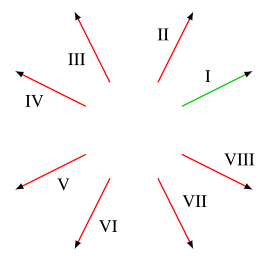
\includegraphics[scale=0.6]{1.png}
\end{center}

(箭头所在象限分别用罗马数字表示)

那么表示方法为($x- und ystep$表示斜率,即渐进步长。):

\begin{center}
    \begin{tabular}{c|c|c|c|c|c|c|c|c}
        Variable &I&II&III&IV&V&VI&VII&VIII\\
        \hline
        \hline
        \textit{swapxy}&false&true&\textbf{true}&false&false&true&true&false\\
        \hline
        \textit{xstep}&1&1&1&-1&-1&-1&-1&1\\
        \hline
        \textit{ystep}&1&1&-1&1&-1&-1&1&-1
    \end{tabular}
\end{center}

描述为代码则是:

\begin{lstlisting}
    if dx < dy then swapxy <- true else swapxy <- false end if
    if x0 < x1 then xstep <- 1 else xstep <- -1 end if
    if y0 < y1 then ystep <- 1 else ystep <- -1 end if
\end{lstlisting}

\subsection{Bresenham-Verfahren}

verwendet ausschließlich Integer-Arithmetik: Addition und Multiplikation mit 2 (Bit-Shift). 

仅使用整数算术:加法和乘以2(位移)

\noindent Voraussetzungen: 

arbeitet direkt mit Integer-Pixelkoordinaten $\Rightarrow$ Start- und Endpunkt müssen auf Pixelzentren liegen.

直接与整数像素坐标一起使用$\Rightarrow$起点和终点必须在像素中心
\\
\\
\noindent Prinzip:

inkrementelle Auswertung der Liniengleichung 线方程的增量评估

\indent\indent aktuelle Position $(x_p, y_p)$, Übergang zu $x_p$ + 1

wähle unter den zwei potentiellen Nachfolgern denjenigen, der Linie am nächsten liegt 

在两个潜在继任者中,选择最接近家族的一个

\indent\indent E (east): ($x_p$ + 1, $y_p$)

\indent\indent NE (north east): ($x_p$ + 1, $y_p$ + 1)
\\
\\
\noindent\textit{In 5 Schritten zum Bresenham-Algorithmus}

1. Inkrementelle Auswertung der Liniengleichung 线性方程式的增量评估

\indent\indent $y(x) = mx + n$

\indent\indent $y(x+1) = m(x+1) + n = y(x) + m$

2. Akkumulieren des Abstands 累积距离

\indent\indent Variable $d$ für (vorzeichenbehafteten) Abstand Pixelzentrum - Linie 

\indent\indent 变量$ d $用于像素中心与线之间的(有符号)距离

\indent\indent einen Schritt nach rechts: $d$ erhöht sich um Anstieg $m$ 

\indent\indent 向右走一步:$ d $增加$ m $

\indent\indent falls $d\geq\frac{1}{2}$: nach oben gehen, $d$ verringert sich wieder um 1 Pixel

\indent\indent 如果 $ d\geq \frac {1} {2} $:上升,$ d $再次减少1个像素

\begin{center}
    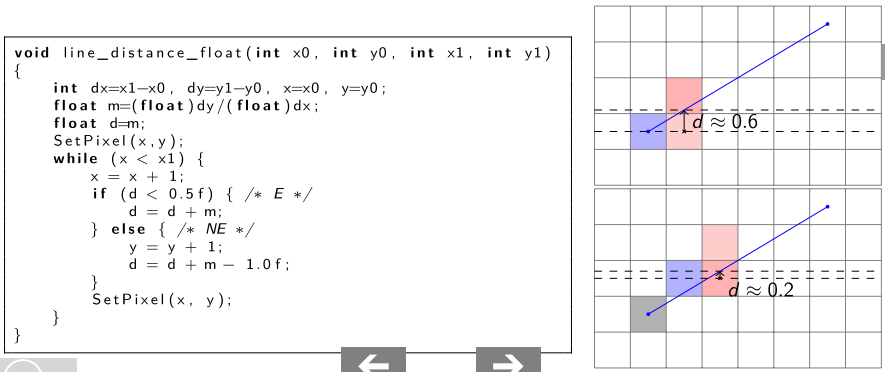
\includegraphics[scale=0.45]{3.png}
\end{center}

3. Vermeiden von Fließkomma-Operationen 避免浮点运算

\indent\indent Einheit von Abstand $d$ bisher Pixel, aber: beliebige Einheit möglich

\indent\indent 距离单位$ d $以前的像素,但是:可能的任何单位

\indent\indent die einzigen Brüche sind m =$\frac{dy}{dx}$ und $\frac{1}{2}$ (Vergleich) $\Rightarrow$ Skalieren des Abstandswerts um $2dx$

\indent\indent 唯一的分数是m = $ \frac {dy} {dx} $和$ \frac {1} {2} $(比较)$ \Rightarrow $将距离值缩放$ 2dx $

4. Vermeiden des Vergleichs mit einer Variablen 避免与变量进行比较

\indent\indent bisher: $d$ = 0 bedeutet, dass Pixelzentrum genau auf Linie liegt, erfordert Vergleich $d < dx$

\indent\indent 先:$ d $ = 0表示像素中心正好在线上,需要比较$ d <dx $

\indent\indent effizienter: Vergleich gegen 0 $\Rightarrow$ Verschieben des Nullpunkts um $−dx$ 

\indent\indent\indent (ändert nur Initialwert und Vergleichskonstante)

\indent\indent 效率更高:与0 $ \Rightarrow $进行比较,将零点移动$ -dx $(仅更改初始值和比较常数)

5. Vorberechnen der Inkremente außerhalb der Schleife 预先计算循环外的增量

\indent\indent Bresenham-Algorithmus


\subsection{Rasterisierungsqualität}

\begin{center}
    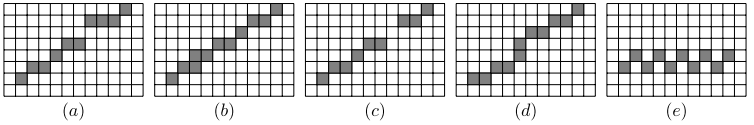
\includegraphics[scale=0.5]{2.png}
\end{center}

\textbf{(a)} Bei jedesmal Schleife wird y um r akkumuliert, wenn es $r\in[0,1]$ keine Sprigen gibt.
在每个循环中,如果没有分支,则y由r累加。

\textbf{(b)} es ist unmöglich, wenn y3 == y2 und y3 == y2 + 1 ist.

\textbf{(c)} Aufgrund jedesmal 1 addierte x wird es jede Spalte 1 Pixel gegeben. Deswegen sollte in X-achse keine Zerbrechen. 
因为x每次都会添加,所以每列有1个像素。 因此,X轴不应断裂。

\textbf{(d)} ähnlich wie (b). Es ist nicht möglich, wenn y5 == y4 und y5 == y4 + 1 ist.

\textbf{(e)} Die Linie ist im Bresenham-Algorithmus immer steigend. D.h. gibt es keine sinkende Möglichkeit.
在Bresenham算法中,这条线一直在上升。 即 没有下沉的可能性。


\subsection{Vorbemerkung: Indexed Rendering 初步:索引渲染}

例如,要处理3个三角形,则需要9个Vertizes。现实中常出现相邻三角形共边的情况。因此不得不在顶点数组Vertex-Array中多次包含绝对相同的顶点,并je einmal für jedes Primitiv。

如左图所示。

\begin{center}
    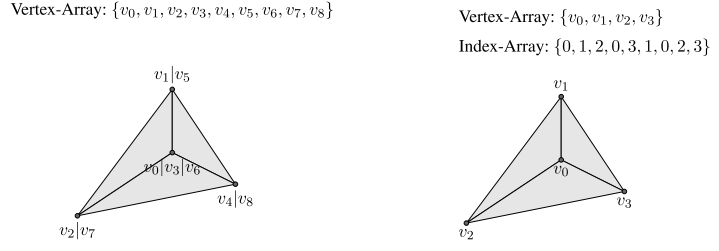
\includegraphics[scale=0.6]{4.png}
\end{center}

右图为\textbf{Indexed Rendering索引渲染},即顶点数组指定所有出现的顶点,但是实际的图元(Primitiv)由附加的索引数组(Array von Indizes)指定。
\\
\\
\textbf{a)} 假设存在一个底面为方形的金字塔,每个顶点有以下属性:

- Position (3D-Koordinaten), beschrieben als 3 $\times$ 32Bit Fließkommazahlen 浮点数字

- Farbe (RGB-Vektor), beschrieben als 3 $\times$ 32Bit Fließkommazahlen

Falls Indexed Rendering zum Einsatz kommt, so soll jeder Index durch einen 32Bit-Integerwert repräsentiert werden. Es sollen nun die folgenden vier Fälle betrachtet werden:

如果使用索引渲染,则每个索引应由32位整数值表示。 现在将考虑以下四种情况:

A: die gesamte Pyramide soll einfarbig blau dargestellt werden

B: die erste Seitenfläche soll rot, die zweite grün, die dritte gelb, die vierte violett und die Grundfläche weiß erscheinen (es soll aber nirgends ein Farbverlauf innerhalb einer Fläche entstehen)

C: die Spitze der Pyramide soll weiß sein, auf jeder der vier Seitenflächen soll ein Farbverlauf von weiß an der Spitze zu blau an der Unterkante entstehen, und die Grundfläche soll einfarbig blau sein

D: die Spitze der Pyramide soll weiß sein, auf jeder der vier Seitenflächen soll ein Farbverlauf von weiß an der Spitze zu blau an der Unterkante erscheinen, und die Grundfläche soll einfarbig grün sein

A:整个金字塔应以蓝色显示

B:第一个侧面应显示为红色,第二个绿色应显示为第三种黄色,第四个紫色应为紫色,而底面应为白色(但在任何区域内均不应出现颜色渐变)

C:金字塔的顶部应该是白色的,在四个侧面的每个侧面上,应该创建从顶部白色到底部边缘蓝色的颜色渐变,并且底部应该是纯蓝色

D:金字塔的顶部应为白色,四个侧面的每一个上均应出现从顶部白色到底部边缘蓝色的颜色渐变,并且底色应为纯绿色

Geben Sie jeweils die \textbf{minimale} Anzahl an Vertizes und Primitiven an, die nötig sind, um den Fall mit und ohne Indexed Rendering umzusetzen, sowie den sich dadurch ergebenden Speicherbedarf (Vertex Array + ggf. Index Array)! (Als Primitivtyp sollen immer Dreiecke verwendet werden.) (6 Punkte)

指定实现带或不带索引渲染的情况所需的最小顶点和图元数量,以及产生的内存要求(顶点数组+可能是索引数组)! (三角形应始终用作基本类型。)
\\
\\
解:

对于非Indexed Rendering,Anzahl Vertizes = $3\times n$,其中$n$为三角形个数。

对于Indexed Rendering,则 = $3\times n - $重复顶点个数。

Anzahl Primitiv = 三角形个数

Speicherbedarf = (Position + Farbe)$\cdot$ Anzahl Vertizes / 8 (Bytes)

\begin{center}
    \begin{tabular}{|c|c|c|c|c|}
        \hline
        Fall&Indexed Rendering&Anzahl Vertizes&Anzahl Primitive&Speicherbedarf(Bytes)\\
        \hline
        A&nein&18&6&432\\
        \hline
        A&ja&5&6&192\\
        \hline
        B&nein&18&6&432\\
        \hline
        B&ja&16&6&408\\
        \hline
        C&nein&18&6&432\\
        \hline
        C&ja&5&6&192\\
        \hline
        D&nein&18&6&432\\
        \hline
        D&ja&9&6&288\\
        \hline
    \end{tabular}
\end{center}

\noindent\textbf{b)} 

Wir betrachten einen Framebuffer in der Auflösung w $\times$ h Pixel. Es soll eine einzelne Linie gerendert werden, wobei ein Standard-Algorithmus zur Linienrasterisierung (Linienbreite ein Pixel, kein AntiAliasing) zum Einsatz komme, z.B. der Bresenham-Algorithmus. 

我们考虑分辨率为w$\times$h像素的帧缓冲区。 使用用于线光栅化的标准算法(线宽一个像素,无抗锯齿)来渲染单条线,例如 Bresenham算法。

Wie hoch ist die minimale und die maximale Anzahl an Fragmenten, die sich beim Rendern ergeben können, wenn Sie Start- und Endpunkt der Linie frei wählen können? Geben Sie für das Minimum und das Maximum jeweils ein Beispiel dafür an, wie Start- und Endpunkt und gewählt werden müssen, um den Fall zu erreichen! (Es genügt, ein Beispielszenario in Worten zu beschreiben, es müssen keine konkreten Koordinaten angegeben werden.) (2 Punkte)

如果您可以自由选择线的起点和终点,那么可以产生渲染的片段的最小和最大数量是多少? 对于最小值和最大值,请举一个示例,说明如何选择起点和终点才能达到目标! (用语言描述示例场景就足够了,不必给出特定的坐标。)
\\
\\
思路:

一个视觉之外的线条,我们可以认为它不存在,因此Minimum=0;

一个视线之内的线条,即屏幕上的某个线条:

1.若这个线条存在,那它必然占有至少1个像素的位置——题目中说了(Linienbreite ein Pixel,kein Anti Aliasin),因此Minimum = 1

2. 在一个屏幕中能够存在最长得到线条是一个位于屏幕对角线的线条,这个线条长度为sqrt(w,h),因此Maximum = sqrt(w,h)
\\
\\
\textbf{c)}

Es werden beginnend ab dem Zeitpunkt $t_0 = 0$ nacheinander 5 Frames einer Animation gerendert. 
 Die Renderzeit der Frames betrage $f_1 = 15ms, f_2 = 10ms, f_3 = 5ms, f_4 = 30ms$ und $f5 = 5ms$.
 Der angeschlossene Monitor arbeite mit eine Bildwiederholfrequenz von 50Hz. 
 Wir gehen vereinfachend davon aus, dass ein Vertical Blanking Interval\footnote{Ein \textit{Vertical Blanking Interval} (deutscher Fachbegriff: \textit{vertikale Austastlücke}) beschreibt die Zeit zwischen der Übertragung der letzen Zeile eines Frames und der Übertragung der ersten Zeile des Folgeframes. 垂直消隐间隔描述了帧的最后一行的传输与下一帧的第一行的传输之间的时间。} unendlich kurz ist, und auch ein \textit{Buffer Swap} keine Zeit verbraucht. Bekannt sei, dass ein Vertical Blanking Intervall zum Zeitpunkt $t_{vblank} = 10ms$ stattfindet. Es sollen drei Fälle betrachtet werden:

从时间t0 = 0开始,动画的5帧一个接一个地渲染。 帧的渲染时间为f1 = 15ms,f2 = 10ms,f3 = 5ms,f4 = 30ms和f5 = 5ms。 连接的显示器以50Hz的刷新率工作。 为简单起见,我们假定垂直消隐间隔无限短,并且缓冲区交换不会消耗任何时间。 已知在时间tvblank = 10ms发生垂直消隐间隔。 应考虑三种情况:

 A: Single-Buffering 单缓冲 (Rendern direkt in den \textbf{FRONT}-Buffer) 
 
 B: Double-Buffering ohne ,,VSync'' 
 
 C: Double-Buffering mit ,,VSync''

Berechnen Sie für die Fälle \textbf{A} bis \textbf{C}, zu welchem Zeitpunkt sich im \textbf{FRONT}-Buffer frühestens Bildteile (nicht notwendigerweise das finale Bild!) von Frame 5 befinden können! (3 Punkte)

对于情况A到C,计算帧5的图像部分(不一定是最终图像!)可以在FRONT缓冲区中的最早时间点!
\\
\\
\indent\indent\indent A: Single-Buffering(Rendern direkt in den FRONT-Buffer)
$$f_1+f_2+f_3+f_4+f_5=65ms$$
\indent\indent\indent B: Double-Buffering ohne ,,VSync''
$$f_1+f_2+f_3+f_4+f_5=65ms$$
\indent\indent\indent B: Double-Buffering ohne ,,VSync''
$$\sum^5_{i=1}20ms\cdot \left\lceil\frac{20ms}{f_i}\right\rceil=120ms$$

\subsection{Lineare Interpolation线性插值}

已知线段$\overline{AB}$的端点$A=\begin{pmatrix}
    -3\\3
\end{pmatrix}$ und $B=\begin{pmatrix}
    6\\0
\end{pmatrix}$. 其颜色值$c_A = (0, 0, 1)$ und $c_B = (1, 0, 1)$。线段上所有其他点的颜色是端点颜色值的线性内插结果(lineare Interpolation der Farbewerte der Endpunkte)。由此能够创建由A到B的颜色渐变。
\\
\\
\textbf{a)} 求线上某点的插值$c$的公式。已知参数$t\in [0, 1]$, so dass bei $t = 0$ der Wert $a$ und bei $t = 1$ der Wert $b$ angenommen wird!

$$\frac{|P-A|}{|B-A|}=\frac{x-x_1}{x_2-x_1}=\frac{y-y_1}{y_2-y_1}=t$$

$$\left\{
    \begin{aligned}
        x=x_1\cdot(1-t)+x_2\cdot t\\
        y=y_1\cdot(1-t)+y_2\cdot t
    \end{aligned}    
\right.\Rightarrow c_P=(1-t)\cdot c_A +t\cdot c_B,\,t\in[0,1]$$

$$= c(t) = c_A + t\cdot(c_B − c_A), t \in [0, 1]$$
\\
\\
\textbf{b)} 
Berechnen Sie den Farbwert des Linienpunktes $C=\begin{pmatrix}
    3\\1
\end{pmatrix}$. 计算线点C的颜色值。

$$t=\frac{\sqrt{(3-(-3))^2+(1-3)^2}}{\sqrt{(6-(-3))^2+(0-3)^2}}=\frac{2\sqrt{10}}{3\sqrt{10}}=\frac{2}{3}$$

$$c(\frac{2}{3})=(0,0,1)+\frac{2}{3}(1,0,0)=(\frac{2}{3},0,1)$$
\\
\\
\textbf{c)}
Der auf der Linie befindliche Punkt $D$ habe den Farbwert $c_D = (\frac{1}{6},0,1)$. Berechnen Sie Koordinaten dieses Punktes! (2 Punkte)
线上的点的颜色值为$c_D$。 计算这一点的坐标!

$$t=\frac{1}{6}$$

$$D=(1-t)\cdot A + t\cdot B = \begin{pmatrix}
    -\frac{3}{2}\\\frac{5}{2}
\end{pmatrix}$$

\subsection{Lineare Interpolation im Dreieck 三角形中的线性插值}

已知三角形顶点$A=\begin{pmatrix}
    3\\1
\end{pmatrix},\,B=\begin{pmatrix}
    11\\1
\end{pmatrix},\,C=\begin{pmatrix}
    7\\7
\end{pmatrix}$. 及其颜色$c_A = (0, 1, 1), c_B = (1, 0, 1)$ und $c_C = (1, 1, 0)$. 
\\
\\
\textbf{a)} 

Gegeben ist ein Punkt $P=\begin{pmatrix}
    7\\3
\end{pmatrix}$. Konstruieren Sie einen Punkt $Q$ auf der Kante $\overline{AB}$, sodass sie den Farbwert des Punktes $P$ durch lineare Interpolation der Farbwerte von $Q$ und $C$ berechnen können. Berechnen Sie dafür den Farbwert des Punktes $Q$ durch lineare Interpolation der Farbwerte von $A$ und $B$, sowie den Finalen Farbwert $c_P$ durch lineare Interpolation von $c_Q$ und $c_P$! (3 Punkte)

给定一个点P.在边缘AB上构造一个点Q,以便可以通过对Q和C的颜色值进行线性插值来计算点P的颜色值。 通过线性插值A和B的颜色值计算点Q的颜色值,以及通过线性插值cQ和cP的最终颜色值cP!

$$\left\{
    \begin{aligned}
        Q=A+t\cdot(B-A)\\
        r\cdot\overrightarrow{CQ}=\overrightarrow{CP}
    \end{aligned}
\right.\Rightarrow t=\frac{1}{2},\,r=\frac{2}{3}$$

$$c_Q=(\frac{1}{2},\frac{1}{2},1)$$

$$c_P=(\frac{2}{3},\frac{2}{3},\frac{2}{3})$$
\\
\\
\textbf{b)}

Die Formeln der linearen Interpolation des Farbwerts von $P$ aus (a) lassen sich umstellen zu der Form:
$c_P=\alpha\cdot c_A+\beta\cdot c_B+\gamma\cdot c_C$. Berechnen Sie $\alpha,\,\beta$ und $\gamma$! (2 Punkte)

可以将(a)中P的颜色值的线性插值公式转换为以下形式:$c_P=\alpha\cdot c_A+\beta\cdot c_B+\gamma\cdot c_C$。求$\alpha,\,\beta$ und $\gamma$.

$$\left\{\begin{aligned}
    c_Q=c_A+t\cdot(c_B-c_A)\\
    c_P=c_C+r\cdot(c_Q-c_C)\\
    c_P=\alpha\cdot c_A+\beta\cdot c_B+\gamma\cdot c_C
\end{aligned}\right.$$
$$\Rightarrow \alpha=\beta=\gamma=\frac{1}{3}$$

\subsection{Baryzentrischen Koordinaten im Dreieck 三角形重心坐标}

Die drei Eckpunkte eines Dreiecks ABC definieren eine Ebene. Baryzentrische Koordinaten erlauben es uns, jeden Punkt dieser Ebene als Koordinatenvektor $(\alpha,\beta,\gamma)$ relativ zum gegebenen Dreieck zu beschreiben:

三角形ABC的三个角点定义一个平面。 重心坐标$(\alpha,\beta,\gamma)$使我们可以将该平面上的每个点描述为相对于给定三角形的坐标向量:

$$P=\alpha A + \beta B + \gamma C \qquad (mit\quad \alpha + \beta + \gamma =1)$$

\begin{center}
    
\includegraphics[scale=0.6]{11.png}
\end{center}

只有当$\alpha,\beta,\gamma$非负数,重心坐标才在三角形内部。

$\alpha=\frac{S_A}{S},\beta=\frac{S_B}{S},\gamma=\frac{S_B}{S}$,其中$S_A,S_B,S_C$为重心与定点的连线将三角形分割成3个部分的面积。

$P=\alpha A + \beta B + \gamma C$可以扩展为插值后:$v=\alpha v_A + \beta v_B + \gamma v_C$, $v$可以是任意属性:Positions, Texture Koordinaten, Farbe, $\vec{n}$, Depth, Material Arrtibute\dots

注:投影后重心坐标会发生变化,因此不能用投影后的图像找重心坐标,而是应先在原图中找到。

$$A_{ABP} = \frac{1}{2} \cdot  |\overline{AB}| \cdot |\overline{P^{'}Q^{'}}|$$
$$A_{ABC} = \frac{1}{2} \cdot  |\overline{AB}| \cdot |\overline{CQ^{'}}|$$
$$\frac{A_{ABP}}{A_{ABC}} = \frac{|\overline{P^{'}Q^{'}}|}{|\overline{CQ^{'}}|} = \frac{|PQ|}{|CQ|}$$
$$\Rightarrow \frac{A_{ABP}}{A_{ABC}} = \frac{|P-Q|}{|C-Q|}$$

\noindent\underline{Flächeninhalt von Dreiecken 三角形面积}

已知三角形顶点$ABC$,确定两个向量:

$$s=\begin{pmatrix}
    s_x\\s_y
\end{pmatrix}=B-A=\begin{pmatrix}
    B_x-A_x\\B_y-A_y
\end{pmatrix}$$
$$t=\begin{pmatrix}
    t_X\\t_y
\end{pmatrix}=C-A=\begin{pmatrix}
    C_x-A_x\\C_y-A_y
\end{pmatrix}$$

Dann berechnet sich der Flächeninhalt des Dreiecks als die Determinante einer Matrix mit den Spalten $s$ und $t$:

然后将三角形的面积计算为具有s和t列的矩阵的行列式:

\begin{equation}
    \begin{aligned}
        A_{ABC} =& \frac{1}{2}det\begin{pmatrix}
            s_x & t_x\\s_y&t_y
        \end{pmatrix}=\frac{1}{2}\begin{vmatrix}
            s_x & t_x\\s_y&t_y
        \end{vmatrix}=\frac{1}{2}(s_xt_y-t_xs_y)\\
        A_{ABC} =& \frac{1}{2}\begin{vmatrix}
            B_x-A_x & C_x-A_x\\ B_y-A_y & C_y-A_y
        \end{vmatrix}=\frac{1}{2}[(B_x-A_x)\cdot(C_y-A_y)-(C_x-A_x)\cdot(B_y-A_y)]
    \end{aligned}
\end{equation}

\begin{center}
    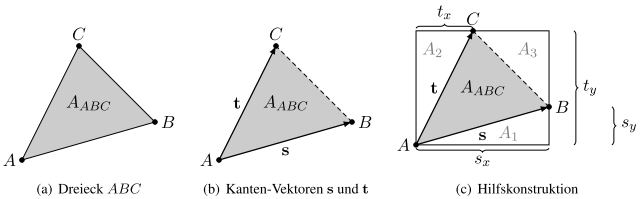
\includegraphics[scale=0.6]{12.png}
\end{center}

\noindent\underline{Baryzentrische Koordinaten im Dreieck 三角形中的重心坐标计算}

已知三角形$ABC$ 和点 $D$, $A=\begin{pmatrix}
    -6\\1
\end{pmatrix},\,B=\begin{pmatrix}
    4\\-1
\end{pmatrix},\,C=\begin{pmatrix}
    2\\5
\end{pmatrix}$ und $D=\begin{pmatrix}
    1\\1
\end{pmatrix}$. 求点$D$相对于三角形$ABC$的重心坐标。

$$A_{ABC} = \frac {1}{2} \cdot 
\begin{vmatrix}
    8 & 10 \\
    4 & -2
\end{vmatrix} = 28\qquad 
A_{CDB} = \frac {1}{2} \cdot 
\begin{vmatrix}
    1 & 3 \\
    4 & -2
\end{vmatrix} = 7
$$$$A_{CDA} = \frac {1}{2} \cdot 
\begin{vmatrix}
    1 & -7 \\
    4 & 0
\end{vmatrix} = 14
\qquad A_{ADB} = \frac {1}{2} \cdot 
\begin{vmatrix}
    -7 & 3 \\
    0 & -2
\end{vmatrix} = 7
$$
$$\Rightarrow \alpha = \frac{1}{4} ,\ \beta = \frac{1}{2} ,\ \gamma = \frac{1}{4}
\qquad \Rightarrow D(\frac{1}{4},\ \frac{1}{2},\ \frac{1}{4})$$
\\
\\
\noindent\underline{Anwendung der baryzentrischen Koordinaten 重心坐标的应用}

\begin{center}
    
\includegraphics[scale=0.6]{13.png}
\end{center}

\noindent\textbf{a)} 

Ordnen Sie den Punkten $P, Q, R$ und $S$ die folgenden absoluten baryzentrischen Koordinaten bzgl. des Dreiecks $ABC$ zu:
$W_1=(\frac{3}{4},\frac{1}{8},\frac{1}{8}),\,W_2=(\frac{1}{4},\frac{1}{4},\frac{1}{2}),\,W_3=(1,-\frac{1}{2},\frac{1}{2}),\,W_4=(0,\frac{1}{3},\frac{2}{3})$ (4p)
将相对于三角形ABC的以下绝对重心坐标分配给点P,Q,R和S:

$$W_1 \rightarrow P,\ W_2 \rightarrow S,\ W_3 \rightarrow Q,\ W_4 \rightarrow R$$

\noindent\textbf{b)} 

Existieren Punkte für welche alle drei absoluten baryzentrischen Koordinaten negative Werte annehmen? Begründen Sie Ihre Antwort! (2 Punkte)
是否存在所有三个绝对重心坐标都为负的点? 解释你的回答!

$$\alpha + \beta + \gamma = 1$$

Wenn es $\alpha<0,\ \beta<0,\ \gamma<0$ gilt, existiert solche Punkte nicht.

\noindent\textbf{c)} 

Den Eckpunkte des Dreiecks seien die RGB-Farbvektoren $c_A=(0\,\frac{1}{2}\,\frac{5}{6})^T,\,c_B=(1\,1\,0)^T$ und $c_C=(1\,0\,1)^T$ zugeordnet. Berechnen Sie den Farbwert des Punktes $P$ mittels baryzentrischer Interpolation! (2 Punkte)

让RGB颜色矢量$c_A=(0\,\frac{1}{2}\,\frac{5}{6})^T,\,c_B=(1\,1\,0)^T$ und $c_C=(1\,0\,1)^T$分配给三角形的顶点。使用重心插值计算点P的颜色值!

$$c_P=\alpha \cdot c_A + \beta\cdot c_B+ \gamma\cdot c_C$$

三角形面积比如$S_{ABC}=\frac{1}{2}|\overrightarrow{AB}\times\overrightarrow{AC}|$求得。那么将此思路带入到求$\alpha,\beta,\gamma$的公式中即可。

%%%%%%%%%%%%%%%%%%%%%%%%%%%%%%%%%%%%%%%%%%%%%%%%%%%%%%%%%%%%%
%%%%%%%%%%%%%%%%%%%%%%%%%%%%%%%%%%%%%%%%%%%%%%%%%%%%%%%%%%%%%
%%%%%%%%%%%%%%%%%%%%%%%%%%%%%%%%%%%%%%%%%%%%%%%%%%%%%%%%%%%%%
%%%%%%%%%%%%%%%%%%%%%%%%%%%%%%%%%%%%%%%%%%%%%%%%%%%%%%%%%%%%%
%%%%%%%%%%%%%%%%%%%%%%%%%%%%%%%%%%%%%%%%%%%%%%%%%%%%%%%%%%%%%

\section{Computergeometrie}

\noindent\underline{Rotation Matrix}

\noindent 2D:

$R_\theta = \begin{pmatrix}
    cos\theta & -sin\theta&0\\
    sin\theta&cos\theta&0\\
    0&0&1
\end{pmatrix}\qquad
R_{-\theta}=\begin{pmatrix}
    cos\theta & sin\theta&0\\
    -sin\theta&cos\theta&0\\
    0&0&1
\end{pmatrix}\qquad R_{-\theta}=R_\theta^{-1}$

\noindent 3D:

$R_x=\begin{pmatrix}
    1\\
    &cos\theta&-sin\theta\\
    &sin\theta&cos\theta\\
    &&&1
\end{pmatrix}\qquad 
R_y=\begin{pmatrix}
    cos\theta&&sin\theta\\
    &1\\
    -sin\theta&&cos\theta\\
    &&&1
\end{pmatrix}\qquad
R_z=\begin{pmatrix}
    cos\theta & -sin\theta\\
    sin\theta&cos\theta\\
    &&1\\
    &&&1
\end{pmatrix}$

\subsection{Affine Abbildungen}

Gegeben Sei das Rechteck ABCD wie in der Grafik dargestellt (alle Punkte liegen in der Ebene $z$ = 0) sowie die Transformationsmatrix
给定如图所示的矩形ABCD(所有点都位于平面z = 0中)和变换矩阵M。
$M=\begin{pmatrix}
    2&-2&0&1\\
    1&1&0&-5\\
    0&0&-\frac{1}{4}&0\\
    0&0&0&1
\end{pmatrix}$
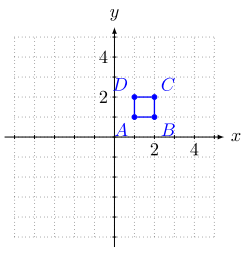
\includegraphics[scale=0.4]{5.png}
\\
\\
\textbf{a)} 

Berechnen Sie die Punkte $A'$ bis $D'$, die sich durch die Anwendung der Transformationsmatrix $M$ auf die Punkte $A$ bis $D$ ergeben, und stellen Sie die Abbildung des Rechtecks in der $xy$-Ebene grafisch dar! (4 Punkte)
计算点$A'$ 到 $D'$,这是将变换矩阵M应用于点A到D的结果,并以图形方式表示矩形在xy平面中的表示!

$A' = M\cdot\begin{pmatrix} 1 \\ 1 \\ 0 \\ 1 \end{pmatrix} =\begin{pmatrix} 1 \\ -3 \\ 0 \\ 1 \end{pmatrix} $
\qquad$B' = M\cdot\begin{pmatrix} 2 \\ 1 \\ 0 \\ 1 \end{pmatrix} =\begin{pmatrix} 3 \\ -2 \\ 0 \\ 1 \end{pmatrix} $

$C' = M\cdot\begin{pmatrix} 2 \\ 2 \\ 0 \\ 1 \end{pmatrix} =\begin{pmatrix} 1 \\ -1 \\ 0 \\ 1 \end{pmatrix} $
\qquad$D' = M\cdot\begin{pmatrix} 1 \\ 2 \\ 0 \\ 1 \end{pmatrix} =\begin{pmatrix} -1 \\ -2 \\ 0 \\ 1 \end{pmatrix} $
\\
\\
\textbf{b)} 

Berechnen Sie die Abbildungen der Einheitsvektoren in $x$- und $y$-Richtung sowie des Koordinatenursprungs, und zeichnen Sie diese ebenfalls in ihre Abbildung aus (a) ein! (3 Punkte)
计算单位向量$x$和$y$方向上的映射以及坐标的原点,并将它们绘制到图片中(a)!

$\vec{e_{x}'} = normiert(M\cdot \vec{e_{x}}) = \frac{1}{5}\cdot \begin{pmatrix} 3 \\ -4 \\ 0 \\ 1 \end{pmatrix}$
\qquad$\vec{e_{y}'} = normiert(M\cdot \vec{e_{y}}) = \frac{1}{\sqrt{17}}\cdot \begin{pmatrix} -1 \\ -4 \\ 0 \\ 1 \end{pmatrix}$

$\vec{e_{z}'} = normiert(M\cdot \vec{e_{z}}) = \frac{4}{\sqrt{417}}\cdot \begin{pmatrix} 1 \\ -5 \\ -\frac{1}{4} \\ 1 \end{pmatrix}$
\qquad$P' = M\cdot \begin{pmatrix} 0 \\ 0 \\ 0 \\ 0 \end{pmatrix} = \begin{pmatrix} 1 \\ -5 \\ 0 \\ 1 \end{pmatrix}$

\subsection{Komposition und Umkehrung von affinen Abbildungen 仿射图的合成和反演}

Gegeben sei eine affine Abbildung M im 3D-Raum, die eine Transformation der Objektpunkte wie in den folgenden Grafiken umsetzt (alle Punkte liegen in der Ebene $z$ = 0):

给定一个3D空间中的仿射映射M,它实现了对象点的转换,如下图所示(所有点都位于平面z = 0中):

\begin{center}
    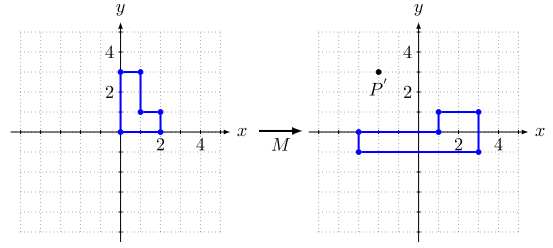
\includegraphics[scale=0.6]{6.png}
\end{center}

\noindent\textbf{a)}
Was ist Transformationsmatrix M?

Skalier mit den Faktoren (1,2,1), dreh um $90^{\circ}$ um die Z-Achse, translatier mit dem Vektor(3,-1,0)$^T$:  

x轴不变,y轴方向放大2倍,逆时针(正方向)旋转$90^{\circ}$,原点移动至(3,-1)。

\begin{center}
    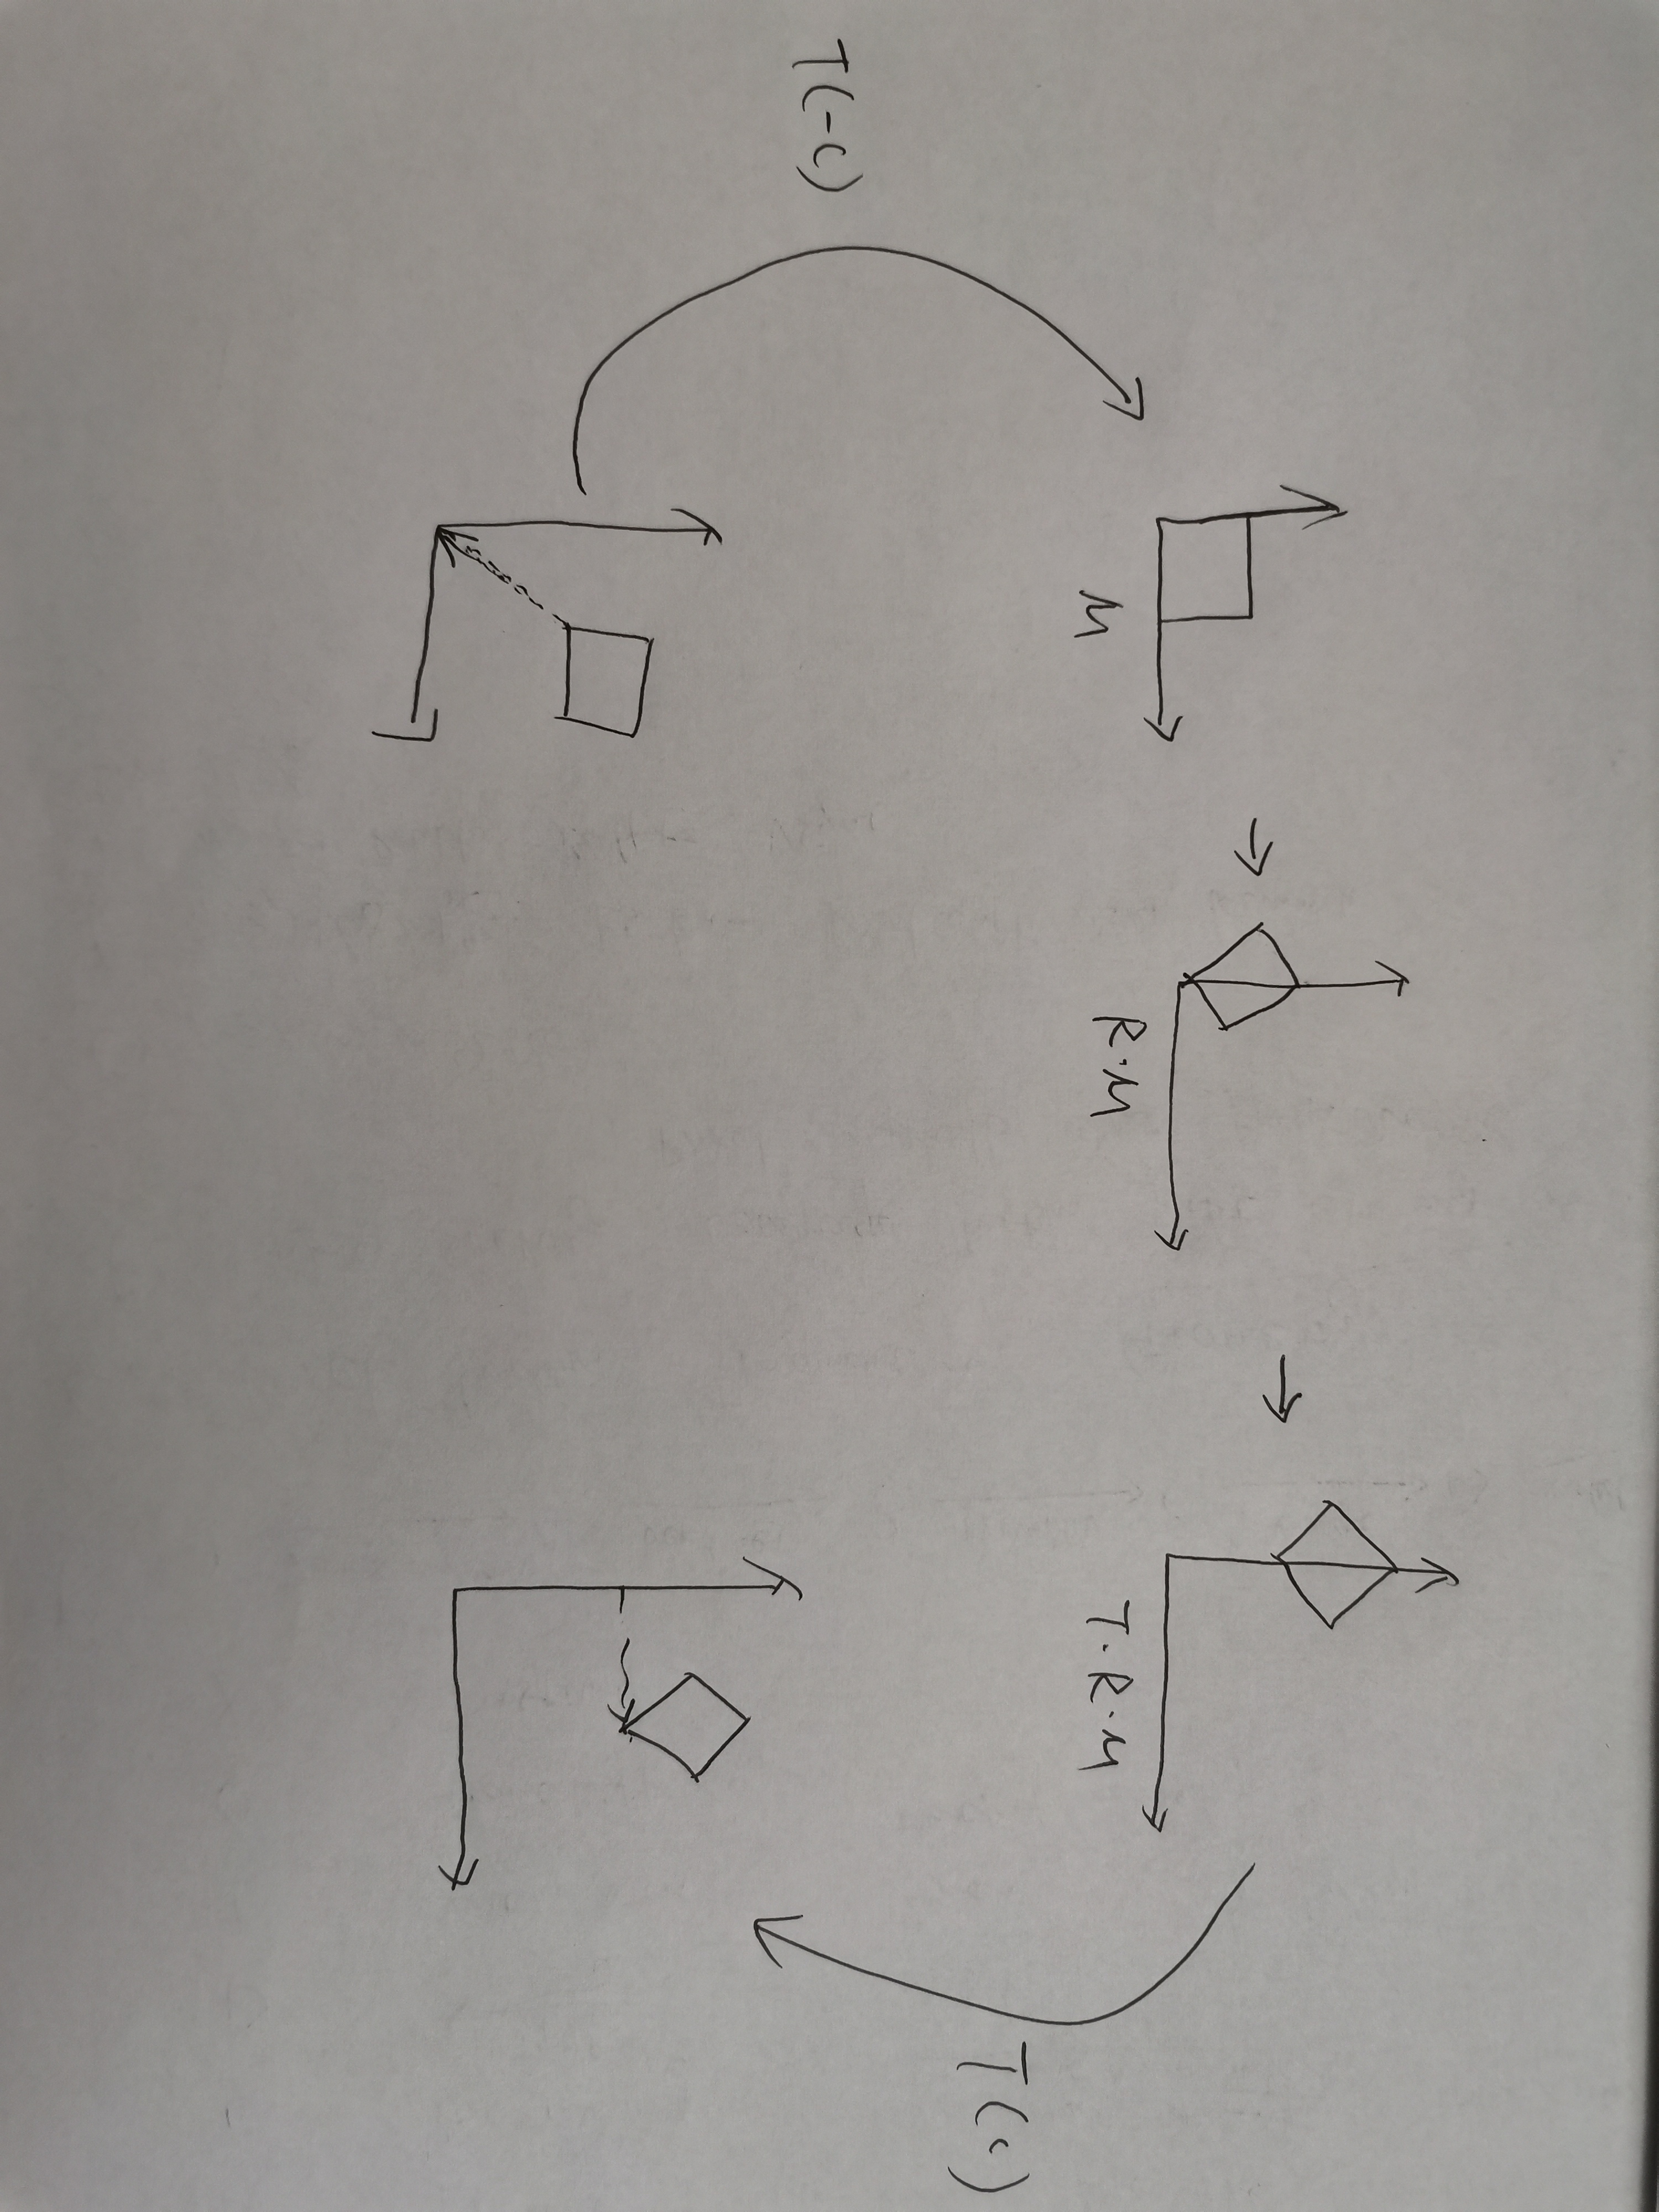
\includegraphics[angle=90,scale=0.1]{7.png}
\end{center}

若要沿“某一点”旋转,需要先平移,使该点成为原点。变换完成后,再平移回来。

$$M_1 = \begin{pmatrix} 1 & 0 & 0 & 0 \\ 0 &2&0&0\\ 0&0&1&0 \\ 0&0&0&1 \end{pmatrix}, M_2 = \begin{pmatrix} cos90^{\circ} & -sin90^{\circ} & 0 & 0 \\ sin90^{\circ} &cos90^{\circ}&0&0\\ 0&0&1&0 \\ 0&0&0&1 \end{pmatrix}, M_3 = \begin{pmatrix} 1 & 0 & 0 & -3 \\ 0 &1&0&-1\\ 0&0&1&0 \\ 0&0&0&1 \end{pmatrix}$$

$$M = M_1 \cdot M_2 \cdot M_3 = \begin{pmatrix} 0 & -2 & 0 & 3 \\ 1 &-2&0&-1\\ 0&0&1&0 \\ 0&0&0&1 \end{pmatrix}$$

\noindent\textbf{b)} 求$M^{-1}$,以及原本的$P$点坐标。

$$M^{-1} = \frac{Adj.A}{det(A)} = \begin{pmatrix} -1 & 1 & 0 & 4 \\ -\frac{1}{2} &0&0&\frac{3}{2}\\ 0&0&1&0 \\ 0&0&0&1 \end{pmatrix}$$ 

$$P = M^{-1}\cdot P' = \begin{pmatrix} 3 \\ \frac{5}{2} \\ 0 \\ 1 \end{pmatrix}$$

\subsection{Transformation des Koordinatensystems}

如图所示,由原本的坐标系$K$变为新的坐标系$K'$。 z维度保持不变,即$z'=z=\begin{pmatrix} 0\\0\\1\\0\end{pmatrix}$

\begin{center}
    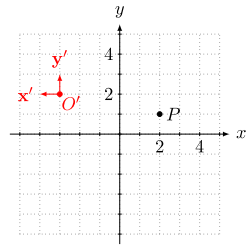
\includegraphics[scale=0.6]{8.png}
\end{center}

求$KOS$变为$KOS'$的Transformationsmatrix $M$,以及新的$P'$坐标。

思路:$KOS$中的原点$O$在$KOS'$中的坐标为$(-3,-2)$,那么需要将原来的$O$点移动至$O'$。并且x轴取负方向,y轴不变。

$$M =\begin{pmatrix} -1 & 0 & 0 & -3 \\ 0 &1&0&-2\\ 0&0&1&0 \\ 0&0&0&1 \end{pmatrix},\qquad
P' = M \cdot P = \begin{pmatrix} -5\\-1\\0\\1 \end{pmatrix}$$

\subsection{Projektionsmatrizen}

\noindent\underline{正交投影 orthogonale Projektion}

\begin{center}
    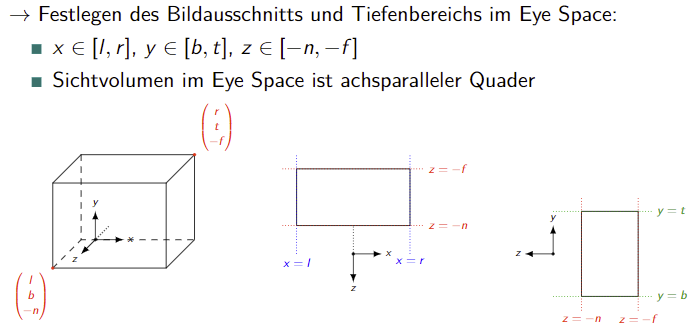
\includegraphics[scale=0.6]{10.png}
\end{center}

$$P_{ortho}=\begin{pmatrix}
    \frac{2}{r-l} & 0&0&-\frac{r+l}{r-l}\\
    0&\frac{2}{r-b}&0&-\frac{t+b}{t-b}\\
    0&0&-\frac{2}{f-n}&-\frac{f+n}{f-n}\\
    0&0&0&1
\end{pmatrix},\,x\in[l,r],\,y\in[b,t],\,z\in[-n,-f]$$

\noindent\underline{透视投影 perspektivische Projektion}

\begin{center}
    
\includegraphics[scale=0.6]{9.png}
\end{center}

$$P_{perspective}=\begin{pmatrix}
    \frac{2n}{r-l}&0&\frac{r+l}{r-l}&0\\
    0&\frac{2n}{t-b}&\frac{t+b}{t-b}&0\\
    0&0&-\frac{f+n}{f-n}&-\frac{2fn}{f-n}\\
    0&0&-1&0
\end{pmatrix}$$

\indent\indent\indent\indent\indent 对称情况下($l=-r, b=-t$):
$$P_{perspective,symmetric}=\begin{pmatrix}
    \frac{n}{r}&0&0&0\\
    0&\frac{n}{t}&0&0\\
    0&0&-\frac{f+n}{f-n}&-\frac{2fn}{f-n}\\
    0&0&-1&0
\end{pmatrix}$$

\noindent\textit{Bsp.}

Gegeben seien die Punkte A bis F mit den Eye-Space-Koordinaten:
$$A=\begin{pmatrix}
    -\frac{9}{5}\\-\frac{9}{10}\\-\frac{9}{5}
\end{pmatrix},\,B=\begin{pmatrix}
    \frac{9}{5}\\-\frac{9}{10}\\-\frac{9}{5}
\end{pmatrix},\,C=\begin{pmatrix}
    \frac{9}{5}\\\frac{9}{10}\\-\frac{9}{5}
\end{pmatrix},\,D=\begin{pmatrix}
    -\frac{9}{5}\\\frac{9}{10}\\-\frac{9}{5}
\end{pmatrix},\,E=\begin{pmatrix}
    -\frac{9}{5}\\-\frac{9}{10}\\-9
\end{pmatrix},\,F=\begin{pmatrix}
    \frac{9}{5}\\-\frac{9}{10}\\-9
\end{pmatrix} $$

sowie die damit beschriebenen Rechtecke(长方形) $ABCD$ und $ABFE$.

Es sollen zwei Fälle betrachtet werden:

\textbf{A:} Orthogonalprojektion mit den Parametern: $l= -\frac{9}{2},\,r= \frac{9}{2},\,b= -\frac{9}{4},\,t= \frac{9}{4},\,n=1,\,f=9$

\textbf{B:} Zentralprojektion mit den Parametern: $l=-1,\,r=1,\,b=-\frac{1}{2},\,t=\frac{1}{2},\,n=1,\,f=9$
\\
\\
\indent\textbf{a)} Stellen Sie die Projektionsmatrizen $P_A$ und $P_B$ auf, die sich entsprechend der Fälle \textbf{A} und \textbf{B} ergeben! (2 Punkte)
根据情况$A$和$B$求投影矩阵$P_A$和$P_B$!

$$
P_A = 
\begin{pmatrix}
    \frac{2}{9} & 0 & 0 & 0 \\
    0 & \frac{4}{9} & 0 & 0 \\
    0 & 0 & \frac{1}{4} & -\frac{5}{4} \\
    0 & 0 & 0 & 1
\end{pmatrix}, 
P_B =
\begin{pmatrix}
    1 & 0 & 0 & 0 \\
    0 & 2 & 0 & 0 \\
    0 & 0 & -\frac{5}{4} & -\frac{9}{4} \\ 
    0 & 0 & -1 & 0
\end{pmatrix}
$$

\textbf{b)} 求$A$和$B$情况下,点$A$至$F$的标准化坐标(normalisierten Gerätekoordinaten)

Fall A: $A' = P_A \cdot A $

$$A' = 
\begin{pmatrix}
    \frac{2}{9} & 0 & 0 & 0 \\
    0 & \frac{4}{9} & 0 & 0 \\
    0 & 0 & -\frac{1}{4} & -\frac{5}{4} \\
    0 & 0 & 0 & 1
\end{pmatrix} \cdot
\begin{pmatrix}
    -\frac{9}{5} \\ -\frac{9}{10} \\ -\frac{9}{5} \\ 1  
\end{pmatrix} = 
\begin{pmatrix}
    -\frac{2}{5} \\ -\frac{2}{5} \\ -\frac{4}{5} \\ 1
\end{pmatrix} 
$$
$$
B' =
\begin{pmatrix}
    \frac{2}{5} \\ -\frac{2}{5} \\ -\frac{4}{5} \\ 1
\end{pmatrix}, 
C'=
\begin{pmatrix}
    \frac{2}{5} \\ \frac{2}{5} \\ -\frac{4}{5} \\ 1    
\end{pmatrix}, 
D'=
\begin{pmatrix}
    -\frac{2}{5} \\ \frac{2}{5} \\ -\frac{4}{5} \\ 1    
\end{pmatrix}, 
E'=
\begin{pmatrix}
    -\frac{2}{5} \\ -\frac{2}{5} \\ 1 \\ 1    
\end{pmatrix}, 
F'=
\begin{pmatrix}
    \frac{2}{5} \\ -\frac{2}{5} \\ 1 \\ 1    
\end{pmatrix}
$$

Fall B: $A' = P_B \cdot A $
$$
A'=
\begin{pmatrix}
    -\frac{9}{5} \\ -\frac{9}{5} \\ 0 \\ \frac{9}{5}    
\end{pmatrix},
B'=
\begin{pmatrix}
    \frac{9}{5} \\ -\frac{9}{5} \\ 0 \\ \frac{9}{5}    
\end{pmatrix},
C'=
\begin{pmatrix}
    \frac{9}{5} \\ \frac{9}{5} \\ 0 \\ \frac{9}{5}    
\end{pmatrix},
D'=
\begin{pmatrix}
    -\frac{9}{5} \\ \frac{9}{5} \\ 0 \\ \frac{9}{5}    
\end{pmatrix},
E'=
\begin{pmatrix}
    -\frac{9}{5} \\ -\frac{9}{5} \\ 9 \\ 9    
\end{pmatrix},
F'=
\begin{pmatrix}
    \frac{9}{5} \\ -\frac{9}{5} \\ 9 \\ 9    
\end{pmatrix}
$$

\subsection{Parametrisierung eines symmetrischen View Frustums 对称视图视锥的参数化}

Die Spezifikation des View-Frustums über die 6 Parameter $l, r, b, t, n$ und $f$ ist meist sehr unintuitiv. Im Falle einer perspektivischen Projektion mit einem symmetrischen Frustum (d.h. wenn der Betrachter mittig vor der Projektionsfläche platziert ist, was im Normalfall angenommen wird) wird das Sichtvolumen meist durch 4 intuitivere Parameter beschrieben:

通过6个参数$l,r,b,t,n, f$来指定视锥的视图非常不直观。 对于具有对称视锥面的透视投影(即通常将观看者放置在投影表面前面的中央位置,通常是假定的),通常用4个更直观的参数来描述视觉体积:

\indent\indent $\circ$ dem Seitenverhältnis $a$, d.h. dem Verhältnis $\frac{Breite}{Hoehe}$ der Fläche, auf der das Bild ausgegeben werden soll,

\indent\indent $\circ$ Seitenverhältnis 长宽比 $a=\frac{Breite}{Hoehe}$

\indent\indent $\circ$ dem \textbf{vertikalen} Oeffnungswinkel $\theta$ (engl. \textit{field of view angle} bzw. kurz \textit{FOV}),

\indent\indent $\circ$ 垂直$FOV$ $\theta$

\indent\indent $\circ$ dem Abstand $n$ zur Near-Plane (in Blickrichtung) und

\indent\indent $\circ$ 到近平面的距离$ n $(在视线方向上)

\indent\indent $\circ$ dem Abstand $f$ zur Far-Plane (in Blickrichtung).

\indent\indent $\circ$ 到远平面的距离$ n $(在视线方向上)

Aus diesen Parametern können die 6 Parameter für ein allgemeines View Frustum bestimmt werden.

可以从这些参数中确定用于普通视锥的6个参数。
\\
\\
\textit{Bsp.}

窗口 720$\times$ 480 Pixeln, $\theta=90^\circ$, $n=2, f=32$。求$l,r,b,t$

\quad \  $a = \frac{720}{480} = \frac{3}{2}$

\quad \  $t = n \cdot tan(\frac{\theta}{2}) = 2tan(\frac{\pi}{2}) = 2$

\quad \  $r = t \cdot a = 2 \cdot \frac{3}{2} = 3$

\quad \  $l = -r = -3, \ b = -t = -2$

\subsection{Wirkungen von Projektionen 投影效果}

有单位立方体 Einheitswürfel投影到2D平面上,判断:

\noindent\textbf{a)} 

Die 2D-Abbildungen aller Kanten, die parallel zur Projektionsebene liegen, sind gleich lang.
平行于投影平面的所有边缘的2D图像的长度相同。

Nur bei Orthogonale Projektion ist es möglich, denn sie parallelprojektion ist, dabei sind all Kanten auf 2D-Abbildung gleich lang.
Dagegen ist es bei zentrale Projektion aufgrund ihrer Differenz der Distanz zweischen verschiedene Kanten und Ursprung nicht möglich.

只有正交投影才有可能,因为它是平行投影,并且二维地图上的所有边长都相同。相反,在中心投影的情况下,由于两个不同的边缘和原点之间的距离不同而无法实现。
\\
\\
\noindent\textbf{b)} 

Die 2D-Abbildungen aller Seitenflächen, die parallel zur Projektionsebene liegen, sind Quadrate.
平行于投影平面的所有侧面的2D图像均为正方形。

Beide sind möglich. Darunter muss die Ursprung (bei Orthogonale Projektion) sich in der Zentrum der Seite befinden.

两者都是可能的。 在此之下,原点(用于正交投影)必须位于页面的中心。
\\
\\
\noindent\textbf{c)} 

Die Flächeninhalt der Abbildung einer Seitenfläche, die senkrecht zur Projektionsebene liegt, ist nicht 0. Begründen Sie Ihre Antworten!
垂直于投影平面的侧面图像的面积不为0.请给出答案!

Nur bei Zentrale Projektion ist es möglich, denn die obene- und untere Edge der Seite auf der Projektionsebene nicht aufeinander, ist die Flächeinheit nicht 0.
Bei Orthogonale Projektion: Wenn die Seiten senkrecht zur Projektionsebene ist, ist die Abbildung der Seite eine Gerade, deswegen nicht möglich.

仅在中心投影时才有可能,因为投影平面上侧面的上下边缘不重叠,所以面积单位不为0。
对于正交投影:如果该侧面垂直于投影平面,则该侧面将显示为直线,因此是不可能的。

\section{Koordinatentransformation}

\subsection{Koordinatentransformation 正向变换}

\begin{center}
    
\includegraphics[scale=0.45]{14.png}
\end{center}



\noindent 已知在\textit{Object Space}中存在三角形$ABC$及其坐标:

$$A_{obj}=\begin{pmatrix}
    -1\\0\\0
\end{pmatrix},\,B_{obj}=\begin{pmatrix}
    1\\0\\0
\end{pmatrix},\,C_{obj}=\begin{pmatrix}
    0\\1\\0
\end{pmatrix}$$

\noindent 以及 Model-Matrix $M$ 和 Projektions-Matrix $P$ :

$$M=\begin{pmatrix}
    0&8&0&6\\
    0&0&1&-2\\
    4&0&0&0\\
    0&0&0&1
\end{pmatrix},\,P=\begin{pmatrix}
    1&0&0&0\\
    0&2&0&0\\
    0&0&-2&-12\\
    0&0&-1&0
\end{pmatrix}$$

\noindent 相机在\textit{World Space}中的坐标为$\begin{pmatrix}
    2\\0\\0
\end{pmatrix}$, 其 $x$轴指向方向$\begin{pmatrix}
    0\\0\\1
\end{pmatrix}$, 其 $y$轴指向方向$\begin{pmatrix}
    0\\1\\0
\end{pmatrix}$ 其 $z$轴指向方向$\begin{pmatrix}
    -1\\0\\0
\end{pmatrix}$.

\noindent 输出窗口(Ausgabe-Fenster)大小为$32\times18$ Pixel,视点(Viewport)为$16\times12$ Pixel,且从像素$\begin{pmatrix}
    4\\4
\end{pmatrix}$开始。

\noindent 可视深度区域(sichtbare Tiefenbereich)映射到\textit{Windows Space}的区间为[0, 1]。
\\
\\
\underline{View Maxtrix $V$}

思路:首先,将原点移动到相机位置(下面V中的第二个矩阵)。然后进行一次基的映射:将$x,y,z$轴的基向量横着写放一块,就构成了下面的第一个矩阵。二者相乘便得到了$V$矩阵。

$$V = 
\begin{pmatrix}
    0 & 0 & 1 & 0 \\
    0 & 1 & 0 & 0 \\
    -1 & 0 & 0 &0 \\
    0 & 0 & 0 & 1
\end{pmatrix} \cdot
\begin{pmatrix}
    1 & 0 & 0 & -2 \\
    0 & 1 & 0 & 0 \\
    0 & 0 & 1 & 0 \\
    0 & 0 & 0 & 1
\end{pmatrix} = 
\begin{pmatrix}
    0 & 0 & 1 & 0 \\
    0 & 1 & 0 & 0 \\
    -1 & 0 & 0 & 2 \\
    0 & 0 & 0 & 1
\end{pmatrix}
$$

\noindent\underline{求点$A$在Clip-, Eye-, ND-, World Space中的坐标}

根据本节开头的图可知计算顺序。

$$A_{ws} = M \cdot A_{obj} = M \cdot \begin{pmatrix} -1 \\ 0 \\ 0 \\ 1 \end{pmatrix} = \begin{pmatrix} 6 \\ -2 \\ -4 \\ 1 \end{pmatrix}\qquad
A_{es} = V \cdot M \cdot A_{obj} = P \cdot A_{ws} =  \begin{pmatrix} -4 \\ -2 \\ -4 \\ 1 \end{pmatrix}$$

$$A_{cs} = P \cdot V \cdot M \cdot A_{obj} = P \cdot A_{es} = \begin{pmatrix} -4 \\ -4 \\ -4 \\ 4 \end{pmatrix}
\qquad A_{nds} = \frac{1}{4} \cdot A_{cs} = \begin{pmatrix} -1 \\ -1 \\ -1 \\ 1 \end{pmatrix}$$

其中$A_{nds}$的值实际上是对$A_{cs}$的标准化,此处写的不够严谨。

\subsection{Umkehrung der Koordinatentransformation 坐标变换的逆}

\begin{center}
    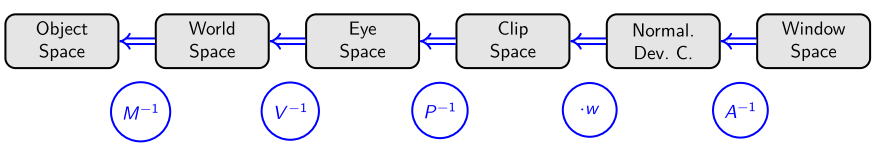
\includegraphics[scale=0.45]{15.png}
\end{center}

\noindent 已知:

$$M=\begin{pmatrix}
    0&-1&0&0\\
    1&0&0&0\\
    0&0&-1&2\\
    0&0&0&1
\end{pmatrix},\,V=\begin{pmatrix}
    0&0&1&0\\
    0&-1&0&0\\
    -1&0&0&2\\
    0&0&0&1
\end{pmatrix},\,P=\begin{pmatrix}
    1&0&0&0\\
    0&2&0&0\\
    0&0&-\frac{3}{2}&-5\\
    0&0&-1&0
\end{pmatrix}$$

$$M^{-1}=\begin{pmatrix}
    0&1&0&0\\
    -1&0&0&0\\
    0&0&-1&2\\
    0&0&0&1
\end{pmatrix},\,V^{-1}=\begin{pmatrix}
    0&0&-1&2\\
    0&-1&0&0\\
    1&0&0&0\\
    0&0&0&1
\end{pmatrix},\,P^{-1}=\begin{pmatrix}
    1&0&0&0\\
    0&\frac{1}{2}&0&0\\
    0&0&0&-1\\
    0&0&-\frac{1}{5}&\frac{3}{10}
\end{pmatrix}$$

$$A_{win}=\begin{pmatrix}
    \frac{5}{2}\\\frac{9}{2}\\0
\end{pmatrix},\,B_{win}=\begin{pmatrix}
    \frac{5}{2}\\\frac{9}{2}\\1
\end{pmatrix}$$

Fenster : $6\times 6$,且铺满(Auflösung von $6\times 6$ Pixel verwendet, und der Viewport fülle dieses Fenster exakt aus.)。

Tiefenbereich : [0,1]。深度映射范围:0处为近平面,1处为远平面。



\noindent\underline{$A$ Matrix}

$$A=\begin{pmatrix}
    \frac{1}{2}v_w&0&0&\frac{1}{2}v_w+v_x\\
    0&\frac{1}{2}v_h&0&\frac{1}{2}v_h+v_y\\
    0&0&\frac{1}{2}(b-a)&\frac{a+b}{2}\\
    0&0&0&1
\end{pmatrix}$$

其中,$v_w$为Fenster的宽度,$v_h$为Fenster的高度。$z_{win}\in[a,b]$,即近平面$a=0$,远平面$b=1$。$(v_x,v_y)$为Fenster左下角的点的坐标,此题为(0,0)
\\
\\
\noindent\underline{Windows Space $\rightarrow$ NDS}

$$A = 
\begin{pmatrix}
    \frac{v_w}{2} & 0 & 0 & \frac{v_w}{2}+v_x \\
    0 & \frac{v_h}{2} & 0 & \frac{v_h}{2}+v_y \\
    0 & 0 & \frac{b-a}{2} & \frac{b+a}{2} \\
    0 & 0 & 0 & 1
\end{pmatrix}=
\begin{pmatrix}
    3 & 0 & 0 & 3 \\
    0 & 3 & 0 & 3\\
    0 & 0 & \frac{1}{2} & \frac{1}{2}\\
    0 & 0 & 0 & 1
\end{pmatrix}
, \
A^{-1}=
\begin{pmatrix}
    \frac{1}{3} & 0 & 0 & -1\\
    0 & \frac{1}{3} & 0 & -1\\
    0&0&2&-1\\
    0&0&0&1
\end{pmatrix}
$$

$$A_{NDS} = A^{-1} \cdot  \begin{pmatrix} A_{win}\\1 \end{pmatrix} =\begin{pmatrix} \frac{-1}{6} \\ \frac{1}{2} \\ -1 \\1 \end{pmatrix}  
\qquad B_{NDS} = A^{-1} \cdot  \begin{pmatrix} B_{win}\\1 \end{pmatrix} =\begin{pmatrix} \frac{-1}{6} \\ \frac{1}{2} \\ 1 \\1 \end{pmatrix}  $$
\\
\\
\underline{$\rightarrow$ Object Space}

\begin{center}
\begin{equation}
    \left\{
        \begin{array}{lr}    
            A_{cs} = w_A\cdot A_{NDS} \\
            A_{es} = P^{-1}\cdot A_{cs} \\
            w_A = 2 \\
            A_{os} = M^{-1} \cdot V^{-1} \cdot A_{es}
        \end{array}
    \right.
\end{equation}
\begin{equation}
    \left\{
        \begin{array}{lr}    
            B_{cs} = w_B\cdot B_{NDS} \\
            B_{es} = P^{-1}\cdot B_{cs} \\
            w_B = 10\\
            B_{os} = M^{-1} \cdot V^{-1} \cdot B_{es}
        \end{array}
    \right.
\end{equation}
\end{center}

$$\Rightarrow A_{os} = \begin{pmatrix} -\frac{1}{2} \\ -4 \\ \frac{7}{3} \\ 1 \end{pmatrix}
,\ B_{os} = \begin{pmatrix} -\frac{5}{2}\\ -\frac{1}{2} \\ \frac{11}{3} \\ 1 \end{pmatrix}$$

\noindent\underline{求Object Space中的交点$Q$,$Q$点为$\overline{AB}$与$xy-Ebene$的交点}

$$A_{os} + r \cdot (B_{os} - A_{os}) = j \cdot \begin{pmatrix} 1 \\ 0 \\ 0 \end{pmatrix} + k\cdot \begin{pmatrix} 0 \\ 1 \\ 0 \end{pmatrix}, \ r = -\frac{7}{4}$$
$$\Rightarrow Q=\begin{pmatrix} 3 \\ -\frac{81}{8} \\ 0 \end{pmatrix}$$

\section{Sichtbarkeit}

\noindent\underline{Backface Culling}

由法面向量确定(如都指向外侧)

\indent\indent Blickrichtungstest

\indent\indent\indent unsichtbare Rückseite, wenn <$\vec{n},\vec{r}$>$\geq 0$ gilt. 其中$\vec{r}$为 Blickrichtung.

\noindent\underline{Tiefensortierung nach Newell}

Vorteil:

$\circ$ 可以处理多边形Polygoneleme

$\circ$ Behandlung aller Sonderfälle

Nachteil:

$\circ$ hoher Rechnenaufwand (bewegte Obj.)

$\circ$ nicht geeignet für den Einsatz innerhalb der Render-Pipeline

$\circ$ nicht geeignet für GPUs

\noindent\underline{Z-Buffer}

只存当前最小值(对于每个Sample (Pixel))

需要额外的深度值缓冲区。

- frame buffer 存储 color values

- depth buffer (z-buffer) 存储 depth

(注:为简单,z始终为正。smaller z $\rightarrow$ closer, larger z $\rightarrow$ further)
\\
\\
\indent Direke im Bildraum lösen.

- speichert pro Pixel einen Tiefenwert

- kann auf Fragment-Ebene Tieftest arbeiten.

Vorteil:

$\circ$ keine Vorerarbeitungsschritte (无需预先处理)

$\circ$ Speicherkomplexität unabhängig von Szenenkomplexität

$\circ$ einfach

$\circ$ von GPU unterstützt

Nachteil:

$\circ$ nicht für transparente Objekte.

$\circ$ begrenzte Präzision(精度) des Tiefpuffers

$\circ$ zusätzlicher Speicherbedarf, Speicherzugriff.

\subsection{Clipping: Cohen Sutherland Algorithmus}

\begin{center}
    \begin{tabular}{c|c|c}
        1001&1000&1010\\
        \hline
        0001&0000&0010\\
        \hline
        0101&0100&0110
    \end{tabular}
\end{center}

4 Bit: 1 wahr, 0 falsch
\\
\\
\indent 0 Bit $x<x_{min}$

1 Bit $x>x_{max}$

2 Bit $y<y_{min}$

3 Bit $y>y_{max}$
\\
\\
\indent Code($P_1$) OR Code($P_2$) = 0000, $\overline{P_1P_2}$ liegt komplett innerhalb

Code($P_1$) AND Code($P_2$) $\neq$ 0000, $\overline{P_1P_2}$ liegt komplett außerhalb

Code($P_1$) AND Code($P_2$) = 0000, 需讨论。

算法见课件07 teil1 - 8



\section{Tiefentest}

\noindent 目的:解决多个三角形先后的问题。
\\
\\
\noindent 有投影矩阵:

$$P_1=\begin{pmatrix}
    \frac{5}{6}&0&0&0\\
    0&-1&0&0\\
    0&0&-\frac{3}{2}&-\frac{1}{4}\\
    0&0&0&1
\end{pmatrix},\,P_2=\begin{pmatrix}
    \frac{5}{6}&0&0&0\\
    0&-1&0&0\\
    0&0&-\frac{5}{2}&-3\\
    0&0&-1&0
\end{pmatrix}$$

Geben Sie für jede der Matrizen die Funktion an,
 die die durch sie definierte Abbildung $z_{ndc}(z_{eye})$ beschreibt! 
 (Dabei sei $z_{eye}$ der Tiefenwert im Eye Space und $z_{ndc}$ der Tiefenwert in 
 normalisieren Gerätekoordinaten.) (2 Punkte)
 为每个矩阵提供描述它们定义的映射zndc(zeye)的函数! (让zeye为眼睛空间中的深度值,让zndc为使设备标准化的深度值。)


 $$F(z) = \frac{f+n}{f-n} + \frac{2\cdot fn}{z(f-n)}$$

 so gilt:
 $$F(z_1) = -\frac{3z_1}{2} - \frac{1}{4}, \ F(z_2) = \frac{5}{2}+\frac{3}{z}$$
 
 
 
Für den Tiefentest werde ein Z-Buffer mit 4Bit vorzeichenlosen Ganzzahlen verwendet. Die Überführung des Tiefenwertes von NDC in den Wertebereich des Z-Buffers erfolge gemäß\footnote{Wir gehen dabei implizit davon aus, dass der NDC-Tiefenwert zunächst vom Intervall [−1, 1] auf einen Window-Space-Tiefenwert im Interval [0, 1] transformiert werde, d.h. $z_{win}(z_{ndc}) = \frac{1}{2}(z_{ndc} +1)$ und dieser dann auf den mit 4 Bit darstellbaren Wertebereich $0, 1, . . . , 2^4 − 1$ für den eigenltichen Buffer abgebildet werde: $z_{buf}(z_{win}) = \lfloor(2^4 − 1)z_{win}\rfloor.$}:
具有4位无符号整数的Z缓冲区用于深度测试。 深度值从NDC到Z缓冲区的值范围的传输根据
 
$$z_{buf}(z_{ndc})=\lfloor\frac{2^4-1}{2}(z_{ndc}+1)\rfloor$$
 
 
深度测试的规则是:只有当片段得到深度值<z缓冲区当前深度值时才会记录。

我们考虑以下两种情况:

\textbf{A:} $z_1=-3,\,z_2=-2$

\textbf{B:} $z_1=-9,\,z_2=-8$

In beiden Fällen liegt $F_2$ im Eye-Space eine Einheit näher am Betrachter als $F_1$.

在这两种情况下,F1都比F1在眼睛空间中更靠近观看者一个单位.

Für den Fall \textbf{A} ergibt sich

mit $P_1$ für $F_1$ : $z_{buf}(z_{ndc}(z_1))=39$, für $F_2$: $z_{buf}(z_{ndc}(z_2))=28$, d.h. $F_2$ besteht den Tiefentest,

计算方法:$z_{ndc}(z_1)=F(z_1)\Rightarrow$ $z_{buf}(F_1(z_1))=\lfloor\frac{2^4-1}{2}(F_1(z_1)+1)\rfloor=39$

mit $P_2$ für $F_1$ : $z_{buf}(z_{ndc}(z_1))=18$, für $F_2$: $z_{buf}(z_{ndc}(z_2))=15$, d.h. $F_2$ besteht ebenfalls den Tiefentest.

Berechnen Sie für den Fall \textbf{B}, ob $F_2$ den Tiefentest bestehen würde,
 jeweils einmal unter Verwendung von $P_1$ und einmal unter Verwendung von $P_2$! 
 Erklären Sie, beim Einsatz welcher Matrix ein Darstellungsproblem auftritt, und beschreiben Sie dieses Problem kurz. (5 Punkte)

 对于情况B,计算一次F2是否通过深度测试,一次使用P1,一次使用P2! 解释在使用时出现显示问题的矩阵,并简要描述问题。

 
 $$\Rightarrow z_{nds}(z_1) = \frac{13}{6}, \ z_{buff}(z_{nds}(z_1)) = 23\frac{3}{4} < z_{buff}(z_{nds}(z_2))=28, \\ z_{nds}(z_2) = \frac{17}{8}$$
 
 Die Verwendung von $P_2$ erhöht sich im Bereich $[-\infty,5]$ langsam. Das Problem ist, dass $z_1,z_2$ eine größe Differenz in eye-Space hat, trotzdem es vielmehr Bit braucht, um zu prüfen.
 
 P2的使用在[-∞,5]范围内缓慢增加。 问题是,即使需要更多的位来检查,z1,z2的眼图空间差异也很大。
 
\subsection{Tiefentest in der Renderpipeline渲染管道中的深度测试}

Wir betrachten einen \textit{Draw Call}, bei dem nacheinander drei Rechtecke $R1,R2$ und $R3$
 (bestehend aus jeweils zwei Dreiecken) gezeichnet werden. 
 Im Object Space seien die Rechtecke alle parallel zur $xy$-Ebene ausgerichtet, 
 lediglich die $z$-Koordinaten der drei Rechtecke unterscheide sich. Als Model-, View- 
 und Projektionsmatrix komme die Einheitsmatrix zum Einsatz, d.h. $M = V = P = I$ 
 und die Object-Space-Koordinaten sind identisch mit den NDC-Koordinaten. 
 Der Viewport entspricht dem gesamten Fenster und die Near Plane werde im Window Space auf 
 $z_{win}$ = 0, die Far-Plane auf $z_{win}$ = 1 abgebildet. 
 Alle drei Rechtecke füllen den Viewport komplett aus. Backface-Culling und Blending sei 
 deaktiviert. Direkt vor dem Draw Call wurde der Color Buffer in jedem Pixel auf 
 schwarz intialisiert, und der Depth Buffer überall auf 1. Der Tiefentest sei aktiviert 
 und auf die Vergleichsrichtung \textbf{kleiner gleich} eingestellt. 
 Der Framebuffer sei 640$\times$480 Pixel groß und wir betrachten das Pixel $p$ mit den Koordinaten 
$p=(400\,\,200)^T$ im Framebuffer.

我们考虑一个绘制调用,其中三个矩形R1,R2和R3(每个由两个三角形组成)一个接一个地绘制。在对象空间中,所有矩形均平行于xy平面对齐,只有三个矩形的z坐标不同。单位矩阵用作模型,视图和投影矩阵,即M = V = P = I,并且对象空间坐标与NDC坐标相同。视口对应于整个窗口,并且在窗口空间中,近平面映射到zwin = 0,远平面映射到zwin = 1。所有三个矩形完全填充了视口。背面剔除和混合禁用。在绘制调用之前,每个像素的颜色缓冲区均初始化为黑色,各处的深度缓冲区均初始化为1,深度测试被激活并设置为小于或等于比较方向。帧缓冲区为640$\times$480像素,我们考虑帧缓冲区中坐标p =$(400\, 200)^T$的像素p。

Während der Ausführung des Draw Calls ergeben sich für das Pixel $p$ eine gewisse Anzahl
 von schreibenden Zugriffen auf den Depth Buffer, und nach dem Draw Call steht im Color 
 Buffer an der Stelle $p$ der Farbwert eines der Rechtecke. Seien $z_1, z_2$ und $z_3$ die 
 \textit{Object Space} $z$-Koordinaten der drei Rechtecke. Diese Werte können innerhalb 
 der folgenden Grenzen gewählt werden: $−1 \leq z_1, z_2, z_3 \leq 1$. Füllen Sie die folgende Tabelle aus:

 在执行绘图调用期间,对像素p的深度缓冲区有一定数量的写访问,并且在绘图调用之后,矩形之一的颜色值在位置p的颜色缓冲区中。 令z1,z2和z3为三个矩形的对象空间z坐标。 可以在以下范围内选择这些值:-1$\leq$z1,z2,z3$\leq$1。 填写下表:

(In den Fällen, in denen die $z$-Werte nicht vorgeben sind, sollen konkrete Zahlenwerte angegeben werden, die zu der geforderten Situation führen. 在未指定$ z $值的情况下,应指定导致所需情况的特定数值。)

\begin{center}
    \begin{tabular}{|c|c|c|c|c|}
        \hline
        \textbf{\#Schreibzugriffe} & \textbf{sichtbares Rechteck}&\qquad$z_1$\qquad\qquad&\qquad$z_2$\qquad\qquad&\qquad$z_3$\qquad\qquad\\
        \hline
        &&0.5&0.6&-0.2\\
        \hline
        &$R_1$&&&\\
        \hline
        3&&&&\\
        \hline
    \end{tabular}
\end{center}

\section{Beleuchtung und Shading}

\subsection{Shading Frequency}

\noindent Flat Shading: 平面着色器。以面为单位,对 面的法向量$\overrightarrow{N}$进行Blinn-Phong计算。快,差。

\noindent Gouraud Shading: Vertex Shader. 利用颜色插值计算。$c=c_0\cdot\alpha+c_1\cdot\beta+c_2\cdot\gamma$。实际上用的是双线性差值 Bilinear Interpolation.

Auswertung der Beleuchtungsgleichung an allen Eckpunkten des Primitivs ,,per-Vertex Lighting''

$\circ$ Umsetzen des Beleuchtungsgleichung im Vertex-Shader,Verwendung der pro Vertex definierten Normalen

$\circ$ 在顶点着色器中实现光照方程式,使用为每个顶点定义的法线

$\circ$ Interpolation des resultierenden FarbwertscalsVaryingsüber das Primitiv

$\circ$ 生成的颜色值标度的插值随基元而变化

Vorteile:

$\circ$ effizient 

$\circ$ schattierte Fläche erscheint weitestgehend glatt (smooth shading) 

$\circ$ Mach-Band-Effekte treten nur dort auf, wo die Intensitätsfunktion ihre Steigung stark ändert

Nachteile:

$\circ$ Glanzlichter (highlights) und Spotlichter werden schlecht reproduziert 

$\rightarrow$ 1 Glanzlicht liegt über einem Vertex: Streuung der Intensität über das gesamte Primitiv 

$\rightarrow$ 2 Glanzlicht im Inneren kann vollständig verschwinden

$\circ$ besonders störend bei Animationen (,,blinkendes'' Glanzlicht)
\\
\\
\noindent Phong Shading: Pixel Shader. 直接用顶点法向量插值。$n=n_0\cdot\alpha+n_1\cdot\beta+n_2\cdot\gamma$,然后用Blinn-Phong。计算之前需注意:顶点法向量求出来之后应先归一化,然后再求插值。

Auswertung der Beleuchtungsgleichung an allen Fragmenten des Primitivs ,,per-Fragment Lighting'' / ,,per-Pixel Lighting''

在原始“每片段照明” /“每像素照明”的所有片段上评估照明方程

$\circ$ Umsetzen des Beleuchtungsgleichung im Fragment-Shader 片段着色器中照明方程的实现

$\circ$ für jedes Fragmentf: Interpolation der Normalennfaus denVertex-Normalen der Eckpunkte 对于每个片段f:从角点的顶点法线插入法线

Bewertung:

$\circ$ schattierte Fläche erscheint weitestgehend glatt 阴影区域显示得尽可能平滑

$\circ$ sehr gute Reproduktion von Glanzlichtern und Spotlichtern 高光和聚光灯的很好再现

$\circ$ vergleichsweise niedrig tesseliertes Modell genügt zur realistischenDarstellung gekrümmter Oberflächen (polygonale Struktur desModells ist nur noch an der Silhouette erkennbar)
一个较低的棋盘格化模型足以真实地表示曲面(模型的多边形结构只能由轮廓识别)

$\circ$ kaum Diskontinuitäten zwischen den Einzelbildern innerhalb einer Animationssequenz
几乎没有动画序列中单个图像之间的任何不连续性

$\circ$ höchster Rechenaufwand aller betrachteten Schattierungsverfahren 考虑到所有着色方法的最高计算量

Phong Shading liefert höchste Bildqualität Phong Shading提供最高的图像质量

$\circ$ Rechenleistung von GPUs mittlerweile ausreichend 现在,GPU的计算能力已足够

$\circ$ umsetzbar mittels programmierbarer Pipeline 可以使用可编程管线来实现

$\Rightarrow$ Phong Shading ist heute das Standard-Shadingverfahren Phong着色是当今的标准着色方法

\subsection{Reflection Model}

\noindent\underline{Blinn-Phone}

\begin{equation}
    \begin{split}
    c_\lambda=&k_{a\lambda}\cdot I_{a\lambda}+&ambienter\, Anteil\\
    &k_{d\lambda}\cdot I_{d\lambda}\cdot max(<\overrightarrow{N},\overrightarrow{L},0>)+&diffuser\, Anteil\\
    &k_{s\lambda}\cdot I_{s\lambda}\cdot u \cdot max(<\overrightarrow{N},\overrightarrow{H},0>)^s&spekularer\, Anteil
    \end{split}
\end{equation}

即光照=环境光+漫反射+高光

\begin{equation}
    u=\left\{
                \begin{array}{lr}
                1 &  \overrightarrow{N}\cdot\overrightarrow{L} >0\\
                0 &  \overrightarrow{N}\cdot\overrightarrow{L} \leq 0
                \end{array}
    \right.
\end{equation}

$$\overrightarrow{L}=\frac{P_l-P_v}{||P_l-P_v||}\qquad \overrightarrow{E}=\frac{P_e-P_v}{||P_e-P_v||}\qquad \overrightarrow{H}=\frac{\overrightarrow{L}+\overrightarrow{E}}{||\overrightarrow{L}+\overrightarrow{E}||}$$

$P_l$: 光源。$P_v$: 当前所求的点。$P_e$: 视点。$\overrightarrow{L}$: (所求点$\rightarrow$光源)入射向量。

$\overrightarrow{E}$: (所求点$\rightarrow$视点)观察向量。$\overrightarrow{H}$: 入射向量与观察向量的平分向量。

$s$: 决定高光范围,s越大,高光越窄,一般取[100,200]。

$k_s$为高光系数,一般取接近“白色”的值。
\\
\\
\noindent Ambient Term 环境光:不取决于任何其他的。$\rightarrow$假设接收到的环境光是恒定的$I_a$。因此环境光是一个常数,把周围的颜色加起来,用以填充黑色阴影部分。
\\
\\
\underline{Phong}

$$L_s=k_s\cdot I_s\cdot max(0,cos\alpha)^p$$

其中$\alpha$为反射光向量$\overrightarrow{R}$与视线向量$\overrightarrow{v}$的夹角。
$p$为衰减系数(控制高光的宽度),大$\rightarrow$窄。离反射光越远,越看不见反射光。
\\
\\
\underline{\textit{Bsp. Diffuser Anteil}}

已知三角形顶点$ABC$和对应的法向量$N_A,N_B,N_C$。光源位于$P_l$,漫反射系数$k_d$,漫反射强度$I_d$。

$$A=\begin{pmatrix}
    -8\\4\\4
\end{pmatrix},\,B=\begin{pmatrix}
    4\\4\\-8
\end{pmatrix},\,C=\begin{pmatrix}
    4\\10\\4
\end{pmatrix},\,N_A=\begin{pmatrix}
    -1\\0\\0
\end{pmatrix},\,N_B=\begin{pmatrix}
    0\\1\\0
\end{pmatrix},\,N_C=\begin{pmatrix}
    0\\0\\-1
\end{pmatrix}$$

$$P_l=\begin{pmatrix}
    0\\12\\0
\end{pmatrix},\,k_d=\begin{pmatrix}
    \frac{1}{2}\\1\\1
\end{pmatrix},\,I_d=\begin{pmatrix}
    1\\0\\\frac{1}{2}
\end{pmatrix}$$

\noindent\textbf{a)} Gouraud Shading:

漫反射光照公式为:$I_d = k_d \cdot l_d \cdot max(<n, \ell  >,0)$

因为需要用到插值,因此接下来需要求$A,B,C$点上的光照分量。
\begin{equation}
    \begin{split}
            I_{dA} & = k_d \cdot l_d \cdot max(<n_A,\ell _A>,0)\\
    &= \begin{pmatrix}\frac{1}{2} \\ 1 \\ 1 \end{pmatrix} \cdot \begin{pmatrix} 1 \\ 0 \\ \frac{1}{2} \end{pmatrix} \cdot max(<\begin{pmatrix} -1 \\ 0 \\ 0 \end{pmatrix},\frac{1}{3}\cdot \begin{pmatrix} 2\\ 2 \\ -1 \end{pmatrix}>,0) \\
        &=0
    \end{split}
\end{equation}

\qquad $I_{dB} = k_d\cdot l_d\cdot max(<n_B,\ell _B>,0) = \frac{2}{3}$

\qquad $I_{dC} = k_d\cdot l_d\cdot max(<n_C,\ell _C>,0) = \frac{2}{3}$

\qquad $I_d = 0\alpha  + \frac{2}{3}\beta + \frac{2}{3}\gamma,\ \alpha + \beta+\gamma = 1,\ \alpha ,\ \beta,\ \gamma \geq 0$
\\
\\
\noindent\textbf{b)} Phong Shading:

该方法使用的是顶点法向量,因此直接将法向量带入插值公式计算即可:

$\vec{n} = \alpha\begin{pmatrix}-1\\0\\0 \end{pmatrix} + \beta\begin{pmatrix}0\\1\\0 \end{pmatrix} + \gamma \begin{pmatrix}0\\0\\-1 \end{pmatrix}=\begin{pmatrix}-\alpha\\\beta\\-\gamma \end{pmatrix}$ 

$I_d = k_d\cdot l_d\cdot max(<\vec{n},\vec{l}>,0)$
\\
\\
\underline{\textit{Bsp. Spekularer Anteil}}

已知:三角形$QRS$,光线照在$\overline{OR}$中间。光源位于$P_l$,镜面光照强度$I_s$,观察者在$P_e$。

$$Q=\begin{pmatrix}
    -1\\-3\\0
\end{pmatrix},\,R=\begin{pmatrix}
    -1+\sqrt{3}\\-3\\0
\end{pmatrix},\,N_Q=\begin{pmatrix}
    0\\1\\0
\end{pmatrix},\,N_R=\begin{pmatrix}
    0\\1\\0
\end{pmatrix}$$

$$P=\frac{1}{2}Q+\frac{1}{2}R=\begin{pmatrix}
    -1+\frac{\sqrt{3}}{2}\\-3\\0
\end{pmatrix},\,P_l=\begin{pmatrix}
    -1\\-2\\0
\end{pmatrix},\,P_e=\begin{pmatrix}
    -1+\sqrt{3}\\-2\\0
\end{pmatrix}$$

$$k_s=\begin{pmatrix}
    1\\1\\1
\end{pmatrix},\,I_s=\begin{pmatrix}
    1\\1\\1
\end{pmatrix},\,s=8$$

\noindent\textbf{a)} Gouraud Shading

高光项公式为:$I_{s}=k_s \cdot l_s \cdot u \cdot max<\vec{n},\vec{h}>^s$


$\overrightarrow{L_Q}=\frac{P_l-Q}{||P_l-Q||}$
, $\overrightarrow{E_Q}=\frac{P_e-Q}{||P_e-Q||}$
$\Rightarrow$ $h_Q = \frac{\overrightarrow{L}+\overrightarrow{E}}{||\overrightarrow{L}+\overrightarrow{E}||}=\frac{1}{\sqrt{7}}\begin{pmatrix}
    \sqrt{3}\\2\\0
\end{pmatrix}$
$\Rightarrow$
$I_{sQ}=\frac{768}{2401}$

同理可得:$I_{sR}=\frac{768}{2401}$

因为题目中要求光刚好打在$\overline{QR}$中间,且$\alpha + \beta +\gamma = 1,$,可得$\alpha = \beta = \frac{1}{2},\gamma = 0$

那么总光照为:$I_s=\alpha\cdot I_{sQ} + \beta\cdot I_{sR}=\frac{768}{2401}$
\\
\\
\noindent\textbf{b)} Phong Shading

直接将顶点法向量带入,则有:

$n=\alpha\cdot N_Q + \beta\cdot N_R$

与前面同理,有$\alpha = \beta = \frac{1}{2},\gamma = 0$。则$\vec{n}=\frac{1}{2}\begin{pmatrix}
    0\\1\\0
\end{pmatrix}+\frac{1}{2}\begin{pmatrix}
    0\\1\\0
\end{pmatrix}=\begin{pmatrix}
    0\\1\\0
\end{pmatrix}$

设照射点$P$已知。

$\overrightarrow{L_P}=\frac{P_l-P}{||P_l-P||}$
, $\overrightarrow{E_P}=\frac{P_e-D}{||P_e-P||}$
$\Rightarrow$ $h_P = \frac{\overrightarrow{L}+\overrightarrow{E}}{||\overrightarrow{L}+\overrightarrow{E}||}=\frac{1}{\sqrt{7}}\begin{pmatrix}
    \sqrt{3}\\2\\0
\end{pmatrix}$

$I_s=I_{sP}=k_s\cdot l_s \cdot u \cdot max(<\vec{n},\vec{h}>,0)^s=\frac{768}{2401}$

\section{Render-Pipeline}

\begin{center}
    
\includegraphics[scale=0.45]{16.png}
\end{center}

\begin{center}
    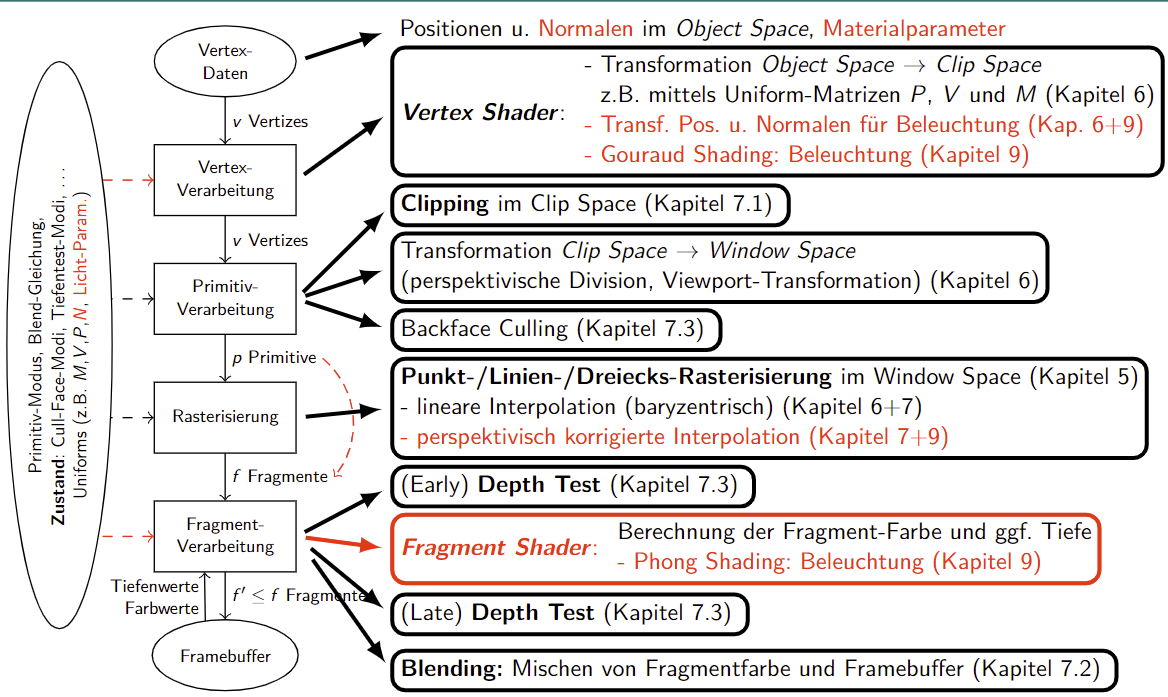
\includegraphics[scale=0.35]{17.png}
\end{center}

\section{Sampling}

利用像素中心对屏幕采样。

可用采样来离散化函数。

\begin{center}
    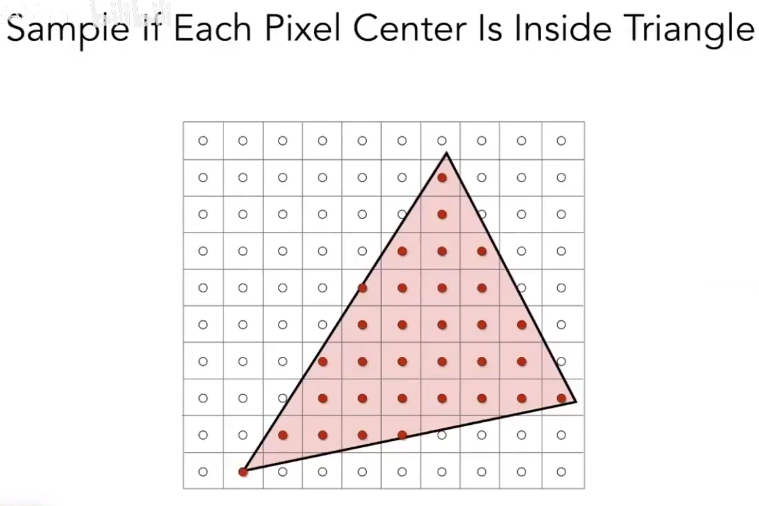
\includegraphics[scale=0.2]{18.png}
    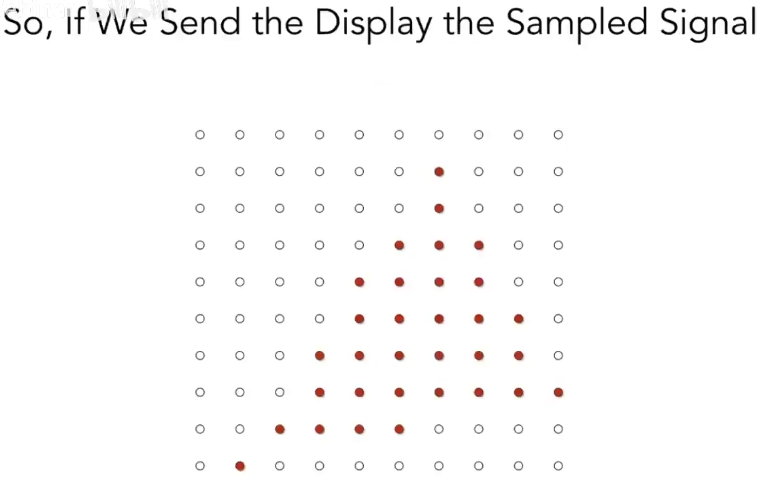
\includegraphics[scale=0.2]{19.png}
\end{center}

Bounding Box: 指左图三角形外一圈的像素集合。

右图可以看到,形成的点阵图像并非是真正的三角形,而是“走样了”的三角形。

\subsection{top-left rule}

Ein Punkt, der auf mindestens einer Dreickskante liegt, wird nur dann als innerhalb des 
Dreiecks betrachtet, wenn er ausschließlich auf top- oderleft-Kanten liegt.

如果至少位于一个三角形边缘上的点仅位于顶部或左侧边缘,则该点仅被视为在三角形内部。

\subsection{Scanline-Verfahrens}

\noindent Vorteile:

inkrementelle Auswertungen auch innerhalb einer Zeile möglich

\indent\indent insbes. Interpolation der Attributwerte

geeignet für Software-Rasterisierung auf CPU

\noindent Nachteile:

in der Praxis Rasterisierungsregeln schwer umsetzbar

\indent\indent die auf der vorherigen Folie angegebenen Intervallgrenzen fürxundysetzen top-left rule theoretisch korrekt um, aber durch begrenzteGenauigkeit der Fließkommadatentypen ergeben sich numerischeProbleme, die dennoch zu Löchern und doppelten Fragmenten angemeinsamen Kanten führen können

Umsetzung ausschließlich mit Integer-Arithmetik möglich, aber aufwendig.

beschränkte Parallelisierbarkeit$\Rightarrow$nicht optimal für GPUs

\subsection{Coverage Samples}

Unter coverage(engl. Abdeckung) eines Primitivs verstehen wir die gesamte von ihm abgedeckte Fläche. Ein Coverage Test ist eine Funktion,die für einen beliebigen Punkt entscheidet, ob dieser innerhalb oder außerhalb des Primitivs liegt.

覆盖图元是指覆盖图元的整个区域。 覆盖率测试是一项功能,它可以确定是否在基元内部还是外部。

\noindent Verfahren:

Coverage Tests für die Zentren aller Pixel, die innerhalb des achsparallelen Begrenzungsrechtecks (axis-aligned bounding box, AABB) des Primitivs liegen.

对位于图元的近轴定界矩形(轴对齐的边界框,AABB)内的所有像素的中心进行覆盖率测试。

\noindent Vorteile

leicht implementierbar

Berechnungen für jedes Pixelvoneinander unabhängig$\Rightarrow$sehr gut parallelisierbar (GPUs!)

每个像素的计算彼此独立$ \Rightarrow $可以很好地并行化(GPU!)

\subsection{Antialiasing 反走样}

\noindent Artifact 瑕疵:

Jaggies - Sampling in space 锯齿(采样太少)

Moire - undersampling images 摩尔纹(采样太多)

Wagon wheel effect - sampling in time 错位轮(信号变的太快而采样跟不上)
\\
\\
\indent SSAA (Super Sampling Anti Alias): most taxing as images are rendered in higher resolution (f.e. 2x SSAA would render a 4k image in 8k resolution, 4x SSAA in 16k and 8x SSAA would render the image in insane 32k).

SSAA(超级采样抗锯齿):当图像以更高的分辨率渲染时(例如2x SSAA将以8k分辨率渲染4k图像,4x SSAA以16k渲染以及8x SSAA会以疯狂的32k渲染图像)最为繁重。


MSAA (Multi Sample Anti Alias): let's call it "optimized SSAA" for simplicity, still nice images but not as taxing as SSAA.

MSAA(多重样本反别名):为简单起见,我们称其为“优化的SSAA”,图像仍然不错,但不如SSAA繁重。


FXAA (Post Process Anti Alias): here the image is processed AFTER it is rendered. As it's a post-process technique it's almost not taxing at all on today's hardware. Depending on the algorithm used (there are differences) images might be a bit blurry to the users eye.

FXAA(后期处理抗锯齿):此处在渲染图像后对其进行处理。由于它是一种后处理技术,因此在当今的硬件上几乎完全不用负担。取决于所使用的算法(存在差异),用户可能会觉得图像有些模糊。
\\
\\
\underline{Antialiasing Idee: Blurring 模糊 (Pre-Filtering) Before Sampling}

\indent\indent Filtering 滤波= Convolution 卷积 (= Averaging 平均)

\begin{center}
    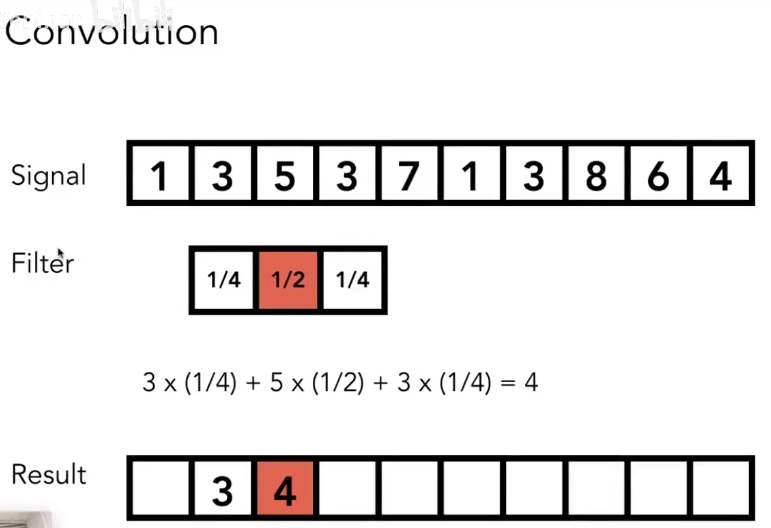
\includegraphics[scale=0.4]{20.png}
\end{center}

\noindent\underline{Supersampling SSAA}

\noindent Prinzip: $n$-faches Sampling innerhalb jedes Pixels

$\circ$ Farbberechnung (Fragment-Shader) erfolgt pro Sample 每个样本进行颜色计算(片段着色器)

$\circ$ Framebuffer speichert pro PixelnSamples 帧缓冲器按像素存储样本

$\circ$ zur Anzeige gemittelter Farbwert aus allen Samples des Pixels 显示像素所有样本的平均颜色值

\indent\indent $\circ$ nachdem komplette Szene gerendert wurde 渲染完整个场景之后  

\begin{center}
    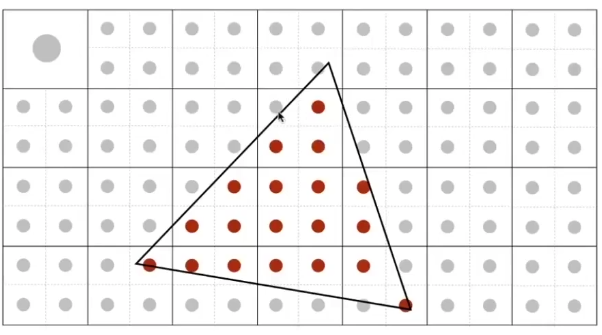
\includegraphics[scale=0.2]{21.png}
\end{center}

此图为SSAA $4\times$,意味着有着$4\times4$倍的计算量。

解决了“模糊”的操作。



Vergleichbar mit Rendern mit höherer Auflösung und anschließendemSkalieren des Bildinhaltes. 可与更高分辨率渲染然后缩放图像内容相媲美

$\circ$ Supersampling flexibler bzgl. der Sampling-Positionen. 关于采样位置的超级采样更加灵活

\begin{center}
    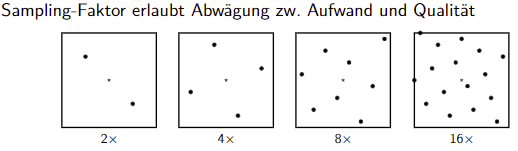
\includegraphics[scale=0.6]{22.png}
\end{center}

\noindent Vorteile:

einfach zu implementieren

\indent\indent insbes. bei Rasterisierung mit Coverage Tests
 
\indent\indent Fixed-Point-Rasterisierer von GPUs erlauben Sampling-Positionen mit Subpixel-Genauigkeit
 
\noindent Nachteile:

hoher Rechenbedarf

\indent\indent hoher Mehraufwand auch für Pixel innerhalb eines Primitives, an denen es eigentlich nicht
\indent nötig ist
 
\indent\indent n-facher Speicherbedarf für den Framebufferebenfalls höherer Bedarf an Speicher-

\indent bandbreite
\\
\\
\underline{Multisampling MSAA}

\noindent Modifikation des Supersampling-Verfahrens:

noch immernCoverage Tests beim Rasterisieren

aber: nur einmaliges Berechnen des Farbwertes (Fragment-Shader),sobald mindestens ein Coverage Test erfolgreich war

\indent\indent Auswerten der Attribute immer für Pixelzentrum(ggf. auch Extrapolation außerhalb des 

\indent\indent Primitivs!)

Übernehmen des Farbwerts in alle Samples, für die der Coverage Testpositiv war

\noindent reduziert Rechenaufwand deutlich, Speicherbedarf bleibt unverändert

benötigte Speicherbandbreite reduziert sich indirekt, falls derFragment-Shader viele Speicherzugriffe benötigt (z.B. Texturierung)

erforderliche Bandbreite dennoch wesentlich höher als ohneAntialiasing

\noindent 修改超级采样方法:

栅格化时仍然进行覆盖率测试

但是:一旦至少一项覆盖率测试成功,就只能进行一次颜色值的计算(片段着色器)\textbf{(默认一个像素内的颜色是均匀的)}

\indent\indent  始终针对像素中心评估属性(可能还在图元之外进行外推!)

颜色值转移到覆盖率测试为positiv的所有样品

\noindent 大大减少了计算量,内存需求保持不变

如果片段着色器需要大量内存访问(例如纹理化),则间接减少所需的内存带宽

所需的带宽仍然比没有抗锯齿的带宽高得多
\\
\\
\underline{Bildbasierte Verfahren, z.B. FXAA}

\noindent Fast Approximate Antialiasing, auch MLAA (Morphological Antialiasing)

\noindent Prinzip:

zuerst normales Rendering 普通渲染优先

Detektion (schräger) Kanten auf finalem Bild 检测最终图像上的(倾斜)边缘

Glättung der Bereiche mit erkannten Kanten 平滑边缘已识别的区域

\noindent Vorteile:

an Objektkanten vergleichbare Ergebnisse wie Multisampling 结果与对象边缘的多重采样相当

kaum zusätzlicher Aufwand 几乎不需要任何额外的努力

gut geeignet für spezielle Renderingtechniken (z.B. deferred shading) 非常适合特殊渲染技术(例如,延迟着色)

\noindent Nachteil: glättet ggf. auch erwünschte Kanten 可能还会平滑所需的边缘

Bild kann generell etwas unscharf wirken 图片通常会显得有些模糊

\section{Texture Mapping 纹理映射}

\subsection{Fragment-Shader: Sampeln der Textur}

$\circ$ pro Vertex sind Texturkoordinaten gegeben oder es existiert eineBerechnungsvorschrift (z.B. Projektion der Objektpunkte auf Ebene,Kugel, Würfel)

$\circ$ 每个顶点都有纹理坐标,或者有一个计算规则(例如,对象点在平面,球体,立方体上的投影)

$\circ$ Koordinaten-Abbildung erfolgt auf derzweidimensionalenProjektionder Primitive, d.h vom Bildraum (in dem die Fragmente platziertsind) in den Texturraum

$\circ$ 坐标映射发生在图元的二维投影上,即从图像空间(其中放置了片段)到纹理空间
\\
\\
Ergebnis des Textur-Samplings kann 纹理采样的结果可以

$\circ$ direkt als Farbwert des Fragments übernommen werden 可以直接用作片段的颜色值

$\circ$ mit der Helligkeit/Farbe aus Beleuchtung/Schattierung kombiniertwerden

$\circ$ 可与照明/阴影的亮度/颜色结合使用

$\circ$ allgemein als Parameter für beliebige pro-Fragment-Berechungendienen

$\circ$ 通常用作任何每片段计算的参数


\subsection{Texel 纹素}

\textbf{Texel} ist die grundlegende Einheit einer Textur in der Computergrafik. \textbf{Texturen} bestehen aus Arrays von Texeln, genauso wie Rastergrafiken als Arrays von Pixeln repräsentiert werden.

纹理像素是计算机图形学中纹理的基本单位。 纹理由纹理像素阵列组成,就像光栅图形表示为像素阵列一样。

\noindent 插值在此处的用处:得到一个在三角形内平滑的过渡。

\subsection{Bilinear interpolation / Bilineare Filterung}

\begin{center}
    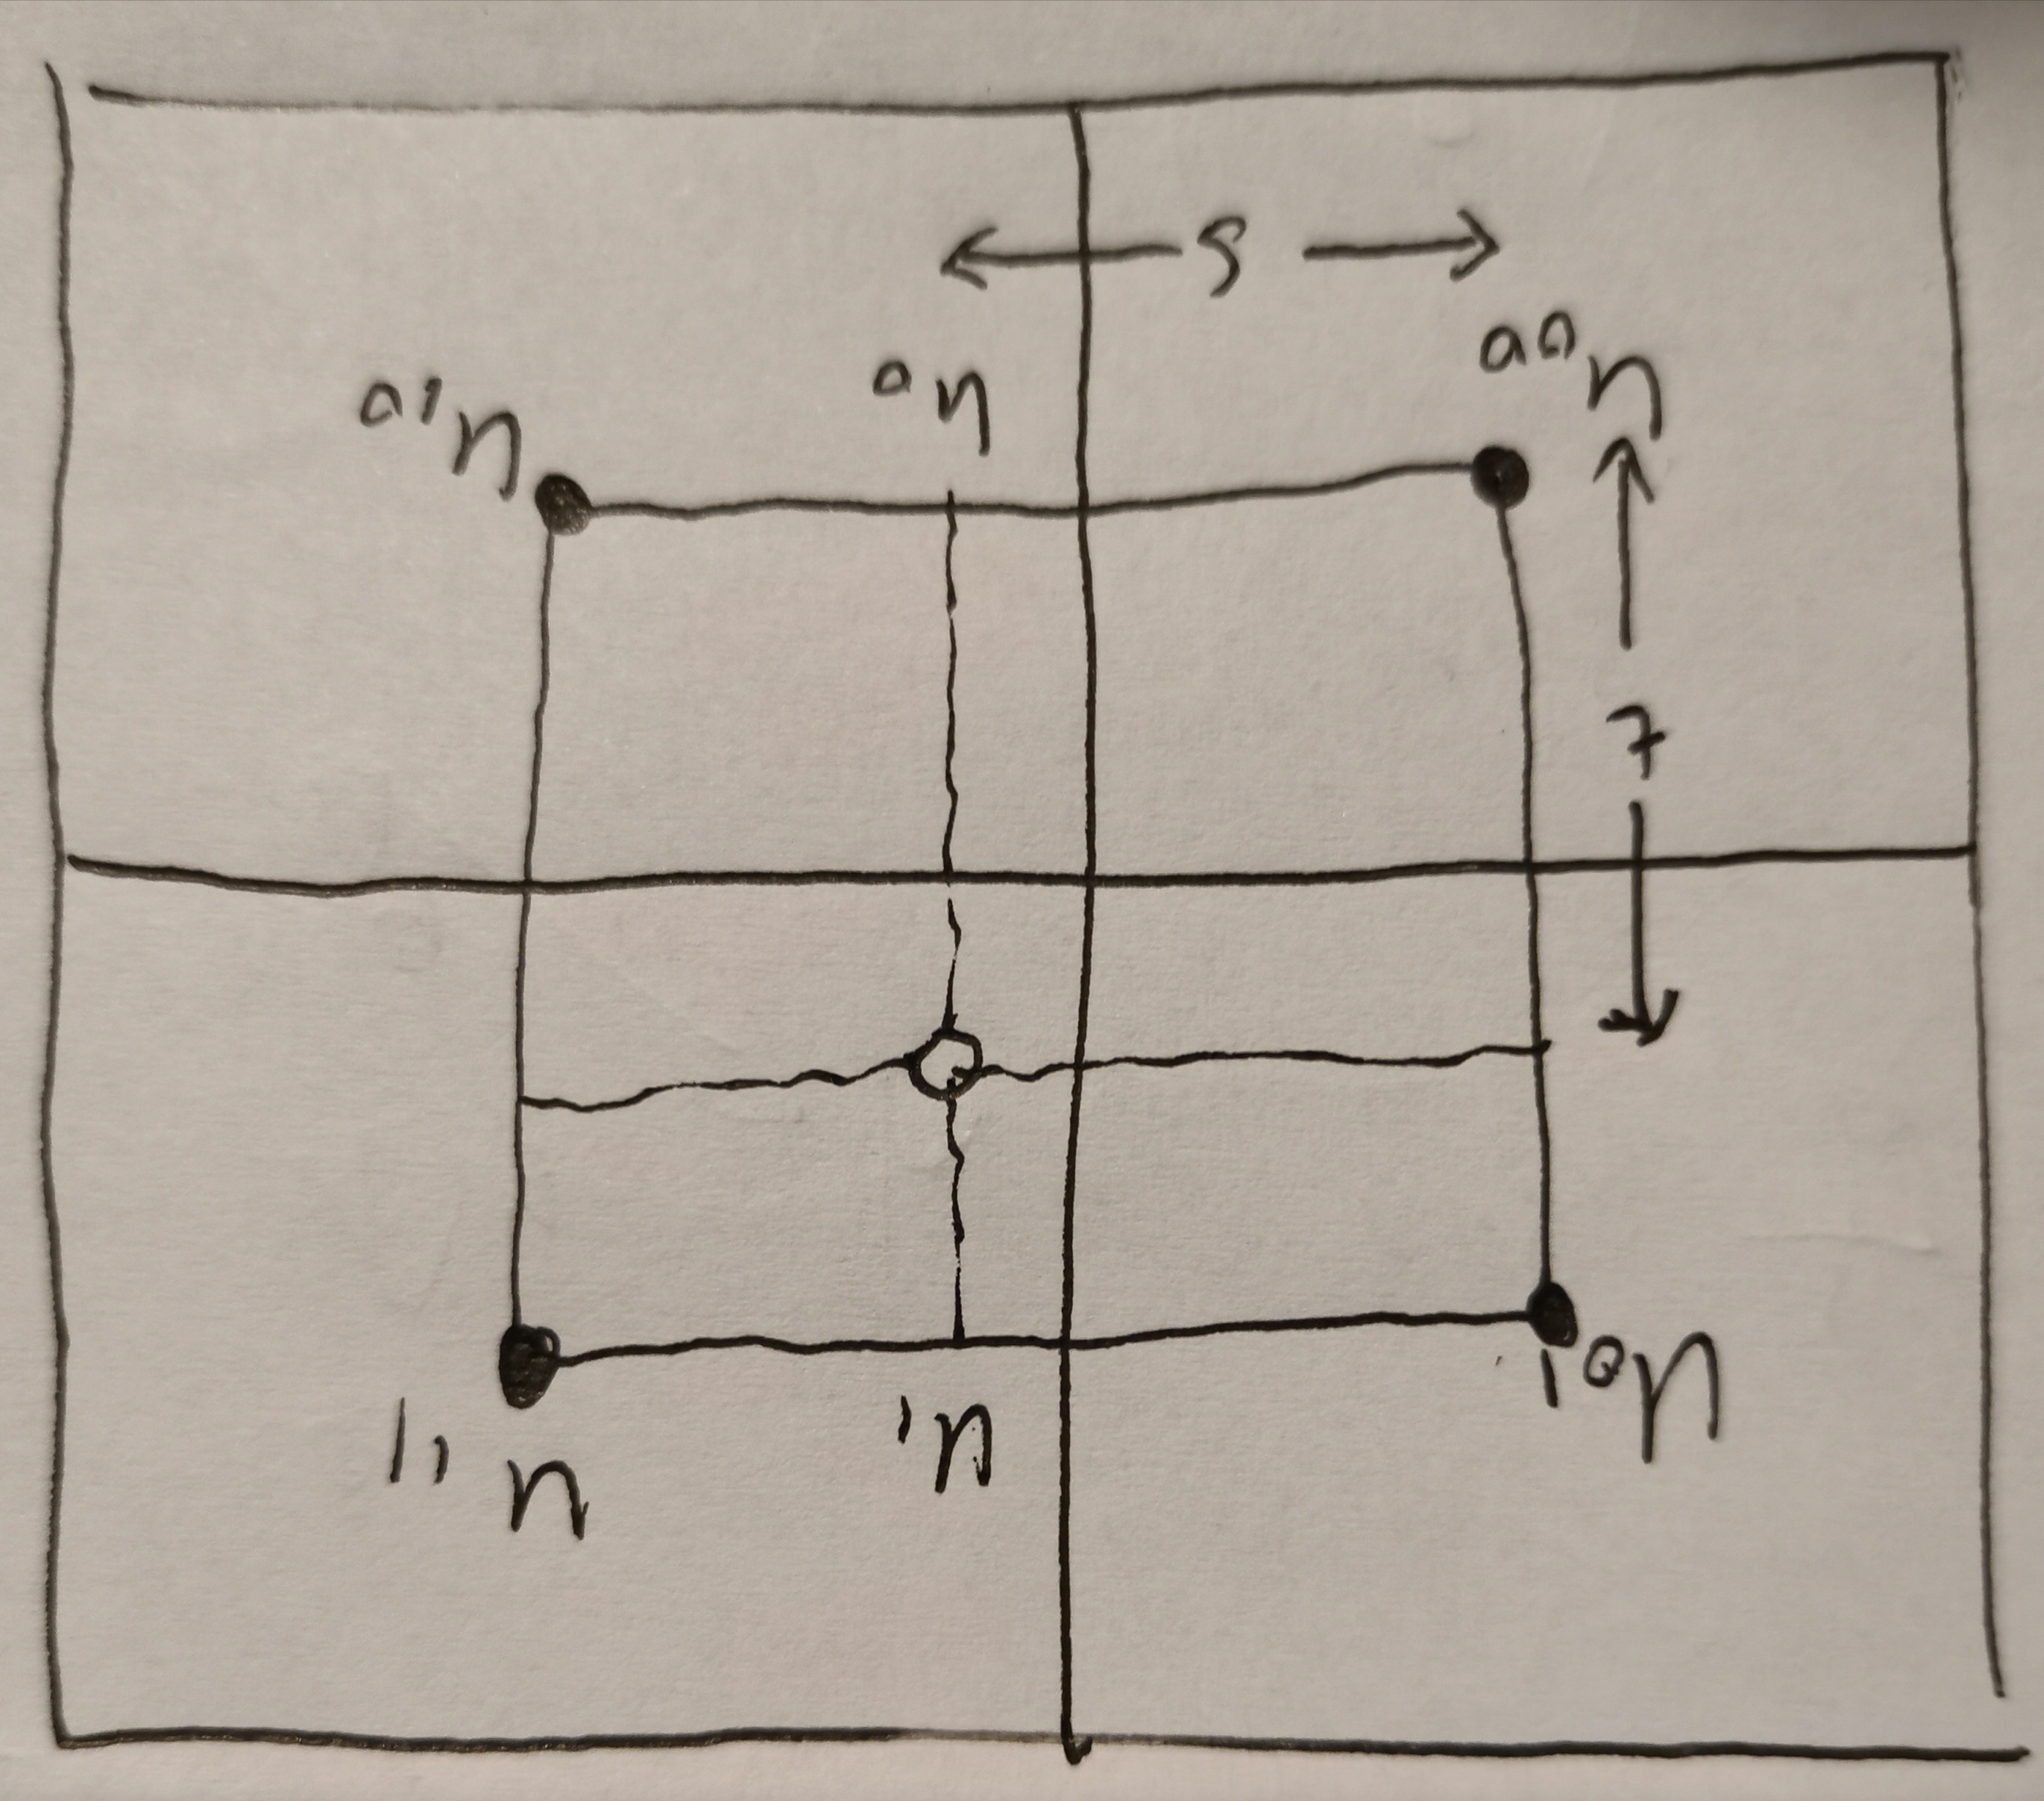
\includegraphics[angle=180,scale=0.05]{23.jpg}
\end{center}

中间白点的坐标为$(x,y)$

\noindent 每4个相邻的Texel进行双线性插值:

1. 定义1D线性插值 linear interpolation 函数$lerp(x,v_0,v_1)=v_0+x(v_1-v_0)$

2. 构造两个辅助线性插值 2 helper lerp:

\indent\indent $u_0=lerp(s,u_{00},u_{10})$

\indent\indent $u_1=lerp(s,u_{01},u_{11})$

3. 最终再计算一次垂直线性插值 final vertical lerp:

\indent\indent $f(x,y)=lerp(t,u_0,u_1)$
\\
\\
\underline{Bicubic interpolation}: 取周围16个Texel.
\\
\\
当纹理分辨率较低,而画面分辨率较高时,会显得模糊,且锯齿明显。

\noindent 当纹理分辨率较高,而画面分辨率较低时,远处会显示出摩尔纹Moire,近处锯齿Jaggies明显。

$\rightarrow$ 近处一个像素覆盖的纹理区域较小,远处一个像素覆盖的纹理区域较大。

若此时采用SSAA会发生什么?

$\circ$ 可以工作,质量高,但costly

$\circ$ 高度缩小后,大多Texel在像素footprint中

$\circ$ 在一个像素中的信号频率太大

$\circ$ 需要更高的采样频率
\\
\\
\indent 因此不采样,而是取区域中的平均值,方法:Mipmap

\subsection{Mipmap}

\noindent Mip-Map Stack: Stapel / Pyramide von Texturen mit jeweilshalbierter Auflösung, bis eine $1\times1$-Textur erreicht ist
以一半的分辨率堆叠/金字塔纹理,直到获得$1\times1$纹理

Stufe (=Mipmap-Level) 0: Originaltextur 级别(= mipmap级别)0:原始纹理

Halbierte Auflösung in jeder Dimension in jeder weiteren Stufe 在每个级别的每个维度上将分辨率减半

in 2D: ein Texel der Stufek+1 repräsentiert einen $2\times 2$ - Block derStufek, einfacher Ansatz: bilde Mittelwert, aber auch aufwendigereBildfilter zur Verkleinerung möglich

在2D模式下:Stufek +1的纹素表示Stufek的$2\times 2$块,简单的方法:取平均值,但也可以使用更复杂的图像过滤器进行缩小

\begin{center}
    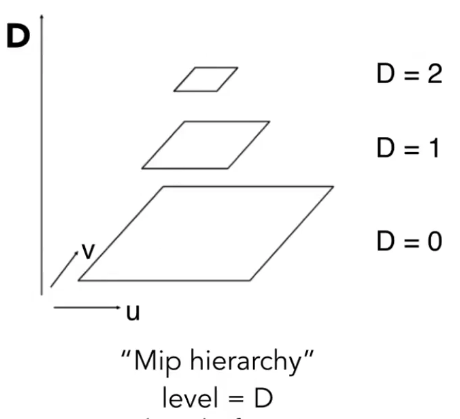
\includegraphics[scale=0.3]{24.png}
\end{center}

第$n+1$层的大小是第$n$层的$\frac{1}{2}$。

Mipmap仅需要原图的$\frac{1}{3}$大小的空间。

\begin{center}
    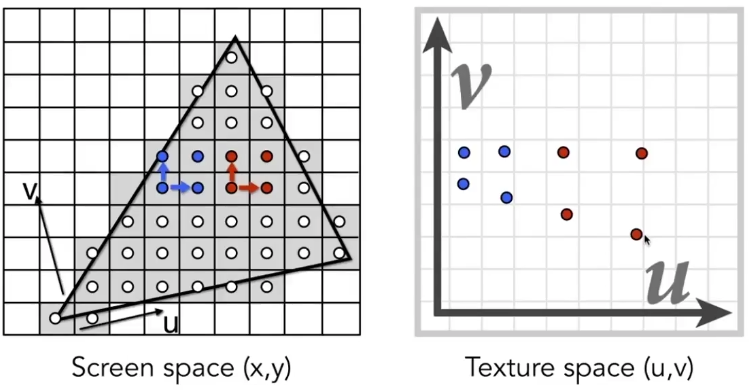
\includegraphics[scale=0.3]{26.png}
    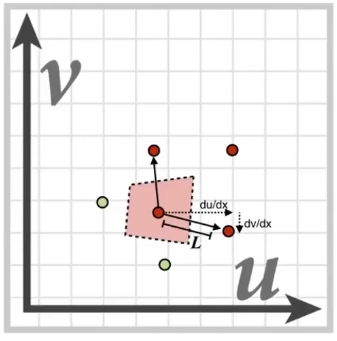
\includegraphics[scale=0.34]{25.png}
\end{center}

左图一个单元为Pixel, 其余两个的单元为Texel。

右图中的$L$为左图中一个色块的边长(即红色区域的边长)。

$D=log_2L$意味着,边长为$L$的区域在$D$层一定会变为一个像素,这一层的值就是这个区域的平均值。

其中$L=max(\sqrt{(\frac{du}{dx})^2+(\frac{dv}{dx})^2},\sqrt{(\frac{du}{dy})^2+(\frac{dv}{dy})^2})$

这样可以极快地查询到所需平均值是多少。
\\
\\
\indent 但层与层之间是离散的,因此想要得到平滑的效果,则需要在层与层之间进行插值,该方法为三线性插值 Trilinear interpolation。
\\
\\
\underline{可能的题目:}

\noindent\textbf{a)} 

Es soll eine $64\times 64$-Textur im RGBA-Format (8 Bit pro Kanal) mit dem Mipmapping-Verfahren gesam-pelt werden. Geben Sie für alle entstehenden Stufen der Mipmap-Pyramide die Auflösung an! BerechnenSie außerdem den Speicherbedarf für die gesamte Pyramide!

将使用mipmapping过程对RGBA格式的$ 64 \times64 $纹理(每个通道8位)进行采样。 输入所有生成的mipmap金字塔级别的分辨率! 还要计算整个金字塔的内存需求!

$$Stufe\,0:64\times64$$
$$Stufe\,1:32\times32$$
$$Stufe\,2:16\times16$$
$$Stufe\,3:8\times8$$
$$Stufe\,4:4\times4$$
$$Stufe\,5:2\times2$$
$$Stufe\,6:1\times1$$

33\% zusatzliche Speicherbedarf.

Speicherbedarf = $64\times64\times4\times8\times1.33=174.326$ Bits
\\
\\
\noindent\textbf{b)}

Das Samplen einer Textur erfolgt für gegebene Texturkoordinaten. Welche Information muss (neben derkompletten Mipmap-Pyramide) zusätzlich noch gegeben sein, damit die Textur mit dem Mipmapping-Verfahren gesampelt werden kann? Begründen Sie Ihre Antwort!

为给定的纹理坐标采样纹理。 还必须提供什么信息(除了完整的mipmap金字塔外),以便可以在mipmapping过程中对纹理进行采样? 解释你的回答!

Abbildung zwischen Bildraum-Punkt$(x,y)$ und Texturkoordinaten($\hat{s},\hat{t}$)damit kann die Kantenl ̈nge ermittelt werden.

在图像空间点$(x,y)$和纹理坐标($ \hat {s},\hat {t} $)之间进行映射,以便可以确定边缘长度。
\\
\\
\noindent\textbf{c)}

Beschreiben  Sie  stichpunktartig  den  trilinearen  Texturfilter  und  erklären  Sie,  welches  Problem  damitgelöst werden soll.

以注释形式描述三线性纹理过滤器,并说明要解决的问题

Umrechnen der Texelkoordinaten Texel坐标的转换

in Kombination mit bilinearer Filterung beim Sampeln beider Mipmap-Stufen. 在对两个mipmap级别进行采样时,与双线性过滤结合使用。

um das Problem, dass es zu sichtbaren ̈Übergängen zwischen den Mipmap-Stufen führt, zu lösen 解决导致在mipmap级别之间出现可见过渡的问题
\\
\\
\underline{存在问题:}

远处的纹理变得完全模糊,被称为overblur: 因为Mipmap计算的是下图中对角线上的图形,即长宽比相同。

\begin{center}
    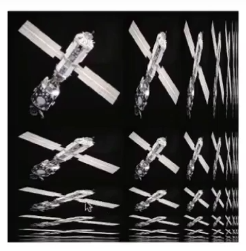
\includegraphics[scale=0.3]{27.png}
\end{center}

Bei starker perspektivischer Verzerrung (Primitive, die flach in die Tiefeorientiert sind) ergeben sich stark unterschiedliche Ausdehnungen des PixelFootprints in horizontaler und vertikaler Richtung.

如果透视畸变严重(基元在深度方向上是平坦的),则像素覆盖区在水平和垂直方向上的扩展程度会非常不同

$\circ$ Mip-Mapping wählt die höchste Stufe (d.h. niedrigste Auflösung)basierend auf der größeren Ausdehnung

$\circ$ Mip映射根据较大范围选择最高级别(即最低分辨率)

$\circ$ für die andere Richtung liegen höher aufgelöste Texturdaten vor, diejedoch nicht genutzt werden können

$\circ$ 在另一个方向上,有较高分辨率的纹理数据,但是不能使用

$\circ$ abgebildete Textur wirkt in einer Dimension verwaschen

$\circ$ 所显示的纹理看起来在一维被洗掉



为解决此问题,方法为:各向异性过滤Anisotropic Filtering / Anisotropischer Texturfilter

\subsection{Anisotropic Filtering / Anisotropischer Texturfilter 各向异性过滤}

\noindent Prinzip: 

statt einem Sample in der höchstmöglichen Stufelog $log_2\lceil \rho\rceil$ gew. Mittel von $n$ Samples in der niedrigeren Stufe $log_2\lceil \frac{\rho}{n}\rceil$.

而不是使用最高级别的日志中的样本log $ log_2 \lceil \rho \rceil $ gew。 较低级别的$ n $个样本的平均值$ log_2 \lceil \frac {\rho} {n} \rceil $。

Wahl vonnanhand des Verhältnisses längerer zu kürzerer Kante $\rightarrow$
hohe Bildqualität, sehr hoher Aufwand

根据长边与短边的比例进行选择$\rightarrow$ 高图像质量,非常费力
\\
\\
\noindent 3倍的开销,因为相比于Mipmap,多了水平和数值方向的计算。这意味着,一个像素在纹理空间中代表的区域是不规则的四边形(即footprint)。

用Mipmap取得的是一个大方块的区域,用Anisotropischer Texturfilter可以取水平或竖直方向上的矩形。

但斜着的矩形仍旧无法很好的解决。
\\
\\
\underline{为了解决斜着的矩形,有比如EWA filtering:}

使用Multiple lookups

加权平均weighted average

Mipmap仍有帮助

可处理不规则的footprints.
\\
\\
\underline{各向异性 $n\times$}

表示算到几层。

in der Praxis typ. Beschränkung auf $n\leq16$

实际上,这通常限于$ n \leq16 $

\subsection{Application of Texture}

Texture = memory + range query (filtering)

$\circ$ 将数据代入段Fragment计算的一般方法。

\subsection{Texture wrapping modes 纹理包装模式}

\noindent\underline{Border}

Border spezifiziert einen (Farb)-Wert,der für alle Koordinaten außerhalb derTextur verwendet wird.

边框指定一个(颜色)值,该值用于纹理之外的所有坐标

\noindent\underline{Clamp}

endlose Weiterführung der äußersten Texelzeilen/ -spalten bzw. diagonal derEcken

最外面的纹素线/列或对角线的无尽连续

\noindent\underline{Repeat}

besonders geeignet für ,,seamless textures'', bei denen Bilddaten an gegenüberliegenden Randkanten zusammenpassen

特别适用于“无缝纹理”,将相对边缘的图像数据放在一起

Verallgemeinerung der Modulo-Operation auf reelle Zahlen 将模运算推广为实数

\begin{center}
    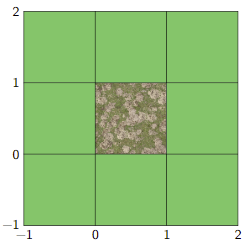
\includegraphics[scale=0.5]{28.png}
    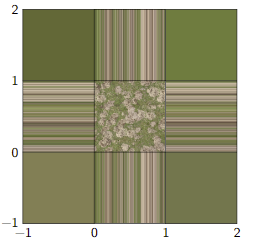
\includegraphics[scale=0.5]{29.png}
    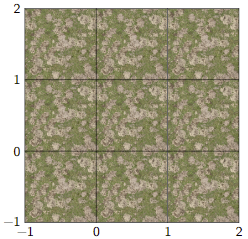
\includegraphics[scale=0.5]{30.png}
\end{center}

\noindent\textit{Bsp.}

已知三角形顶点$ABC$,以及其分配的归一化纹理坐标$c_A,c_B,c_C$,用下图对此三角形进行渲染。

$A=\begin{pmatrix}
    3\\1\\0
\end{pmatrix},\,
B=\begin{pmatrix}
    1\\0\\3
\end{pmatrix},\,
C=\begin{pmatrix}
    0\\3\\1
\end{pmatrix},\,
c_A=\begin{pmatrix}
    \frac{1}{6}\\\frac{1}{6}
\end{pmatrix},\,
c_B=\begin{pmatrix}
    \frac{1}{3}\\\frac{5}{6}
\end{pmatrix},\,
c_C=\begin{pmatrix}
    \frac{5}{6}\\\frac{2}{3}
\end{pmatrix}$

\begin{center}
    
\includegraphics[scale=0.5]{31.png}
\end{center}

在栅格化(Rasterisierung)过程中,将生成一个片段(Fragment),其取样位置(Sample-Position) $S$ 恰好对应于边$\overline{AB}$的中心。RGB模型中的以下颜色矢量分配给纹理像素T1至T9

$T_1=\begin{pmatrix}
    1\\0\\1
\end{pmatrix},\,
T_2=\begin{pmatrix}
    1\\0\\0
\end{pmatrix},\,
T_3=T_8=\begin{pmatrix}
    0\\1\\0
\end{pmatrix},\,
T_4=T_9=\begin{pmatrix}
    0\\1\\1
\end{pmatrix},\,
T_5=\begin{pmatrix}
    0\\0\\1
\end{pmatrix},\,
T_6=T_7=\begin{pmatrix}
    1\\1\\0
\end{pmatrix},\,$

使用Clamp。

\noindent\textbf{a)}

Bestimmen Sie die Texturkoordinaten $c_S$, die dem Punkt $S$ zugeordnet werden müssen! (Sie können davon ausgehen, dass das Dreieck ohne perspektivische Verzerrung abgebildet wird.)

确定必须分配给点$ S $的纹理坐标$ c_S $! (您可以假定所描绘的三角形没有任何透视变形。)

$$c_S=\frac{1}{2}(c_A+c_B)=\begin{pmatrix}
    \frac{1}{4}\\\frac{1}{2}
\end{pmatrix}$$

farbewert von $c_S$ ist gleich $T_4$

\noindent\textbf{b)}

Berechnen Sie den Farbwert, der sich beim Sampeln der Textur an den Koordinaten $c_S$ ergibt, wenn nearest Filtering verwendet wird!

如果使用最接近的滤镜,计算在坐标$ c_S $上对纹理进行采样时得到的颜色值!

$$\tilde{c}_S=\begin{pmatrix}
    \lfloor s_S\cdot w \rfloor\\
    \lfloor t_S\cdot h \rfloor
\end{pmatrix}=\begin{pmatrix}
    0\\1
\end{pmatrix}$$

\noindent\textbf{c)}

Berechnen Sie den Farbwert, der sich beim Sampeln der Textur an den Koordinaten $c_S$ ergibt, wenn ein bilinearer Filter verwendet wird!

如果使用双线性滤镜,则计算在坐标$ c_S $处对纹理进行采样后得出的颜色值!

wähle $T_7,T_8,T_5,T_4$, horizontal: $\alpha$, vertikal: $\beta$

$$S=\beta[(1-\alpha)T_8+\alpha T_7]+(1-\beta)[(1-\alpha)T_5+\alpha T_4],\,\alpha=\frac{3}{4},\,\beta=0$$

Daten einsetzen: $S=\begin{pmatrix}
    0\\\frac{3}{4}\\1
\end{pmatrix}$







































































































\end{document}